\documentclass[conference,letterpaper,onecolumn]{IEEEtran}
%\usepackage[ansinew]{inputenc}
\usepackage{graphicx}
\usepackage{psfrag}\usepackage{stfloats}
%\usepackage[spanish]{babel}
\usepackage{epsfig}
\usepackage{pifont}
\usepackage{amssymb}\usepackage{fixltx2e}
\usepackage{amsmath}
\usepackage{rotate}\usepackage{anysize}
%\usepackage{rotating}
\usepackage{cite}
\usepackage{float}
\usepackage{fancybox}
\usepackage{subfig}

\newcommand{\pig}[1]{\mbox{\boldmath ${#1}$}	}


\newtheorem{Theod}{{\bf Definition}}


\setlength{\oddsidemargin}{5mm}
\setlength{\evensidemargin}{5mm}
\setlength{\topmargin}{4mm}
\setlength{\textwidth}{15cm}
\setlength{\columnsep}{5mm}
\setlength{\textheight}{24cm}

\begin{document}

\title{A thorough explanation of the double bounded homotopy applied to nonlinear circuit simulation}

\author{\authorblockN{H\'ector V\'azquez-Leal}
\authorblockA{Universidad Veracruzana\\
Facultad de Instrumentaci\'on Electr\'onica\\
Xalapa, Veracruz, M\'exico\\
Email: hvazquez@uv.mx}
\and
\authorblockN{Luis Hern\'andez-Mart\'{\i}nez}
\authorblockA{INAOE\\
Departamento de Electr\'onica\\
Email: luish@inaoep.mx}
\and
\authorblockN{Arturo Sarmiento-Reyes}
\authorblockA{INAOE\\
Departamento de Electr\'onica\\
Email: jarocho@inaoep.mx}
\and
\authorblockN{Roberto Casta\~neda Sheissa}
\authorblockA{Universidad Veracruzana\\
Facultad de Instrumentaci\'on Electr\'onica\\
Xalapa, Veracruz, M\'exico\\
Email: rocastaneda@uv.mx}
}


\maketitle

\begin{abstract}
On this work a deep study of the Homotopy method called {\it double bounded Homotopy} is presented. This method shows new and interesting properties like symmetry axis, multiple solution lines, and closed Homotopy paths. The characteristics for this new Homotopy are attractive and can be used as the foundation for a new class, or variety, of Homotopy with similar properties. Finally, several application examples for this Homotopy are provided for the solution of non-linear circuits.
\end{abstract}
 

\section{Introduction}

There are several areas where the efficient and precise solution for non-linear equation systems is a relevant work. For instance, operating point calculation in DC for an electronic circuit is a relevant task performed by circuit simulators since that operating point is employed as the starting point to perform other types of analysis like small signal, transient, and many more. Nevertheless, the task to locate an operating point or several points for non-linear circuits is complex and even commercial circuit simulators fail to converge in a solution. This situation has motivated the research for new methods capable to resolve non-linear equation systems in a more precise and efficient way.

The rapid increase on the number of transistors in an integrated circuit and the increase of complexity for the models (result of lowering the dimension in the components) results in a complex calculation for the equilibrium equation, this leads to two phenomena:  existence of several unexpected operating points  and lack of convergence to the operating point for the Newton-Raphson method (employed in circuit simulators). The existence of multiple operating points generates the need to use other methods, other than the Newton-Raphson, like Homotopy methods. Opposite to the Newton-Raphson method, Homotopy is capable to locate multiple operating points. Besides, the high complexity of the equilibrium equation makes Newton-Raphson, sometimes, unable to converge mainly because this method is locally convergent. Homotopy methods \cite{cont_bra,cont_chu1,cont_hun,homo_jaewook} have been useful to locate multiple operating points and converge to solutions where Newton-Raphson method is not capable.

Several types of Homotopy are employed in electronics. These can be classified in two big groups (see figure \ref{construc}):

\begin{itemize}
\item  Natural parameter Homotopy. This means that Homotopy takes as deforming parameter some circuit variable with physical meaning. Commercial simulators use this kind of Homotopy like: stepping sources, stepping conductances, among others.
\item  Artificial parameter Homotopy. This kind of Homotopy add an extra parameter to the equilibrium equation. It is completely unrelated to the nature of the circuit, that is the reason why is called artificial parameter. Nevertheless, it is possible that an artificial parameter Homotopy has an interpretation or circuital equivalent \cite{homo_ArtificialP}. Some example of this type are: Chua's\cite{cont_chu1}, Chao's\cite{cont_kao}, Branin's\cite{cont_bra}, variable gain\cite{homo_ArtificialP}, variable stimulus \cite{homo_ArtificialP}, fixed point \cite{cont_mix}, modified fixed point\cite{homo_yamamura},
variable dimension\cite{cont_leu1,cont_koya1,cont_yama}, thread\cite{homo_threading}, circuital \cite{homo_ushida1}, multiple parameters\cite{homo_dobletrazado,homo_DWolfMulti}, double bounded Homotopy \cite{homo_iscas05}, BLHOM \cite{BHLHOM}, and constructive Homotopy\cite{homo_jaewook}. 
\end{itemize}

\begin{figure*}[tbp]
\psfrag{L}{$\lambda$}
\centering
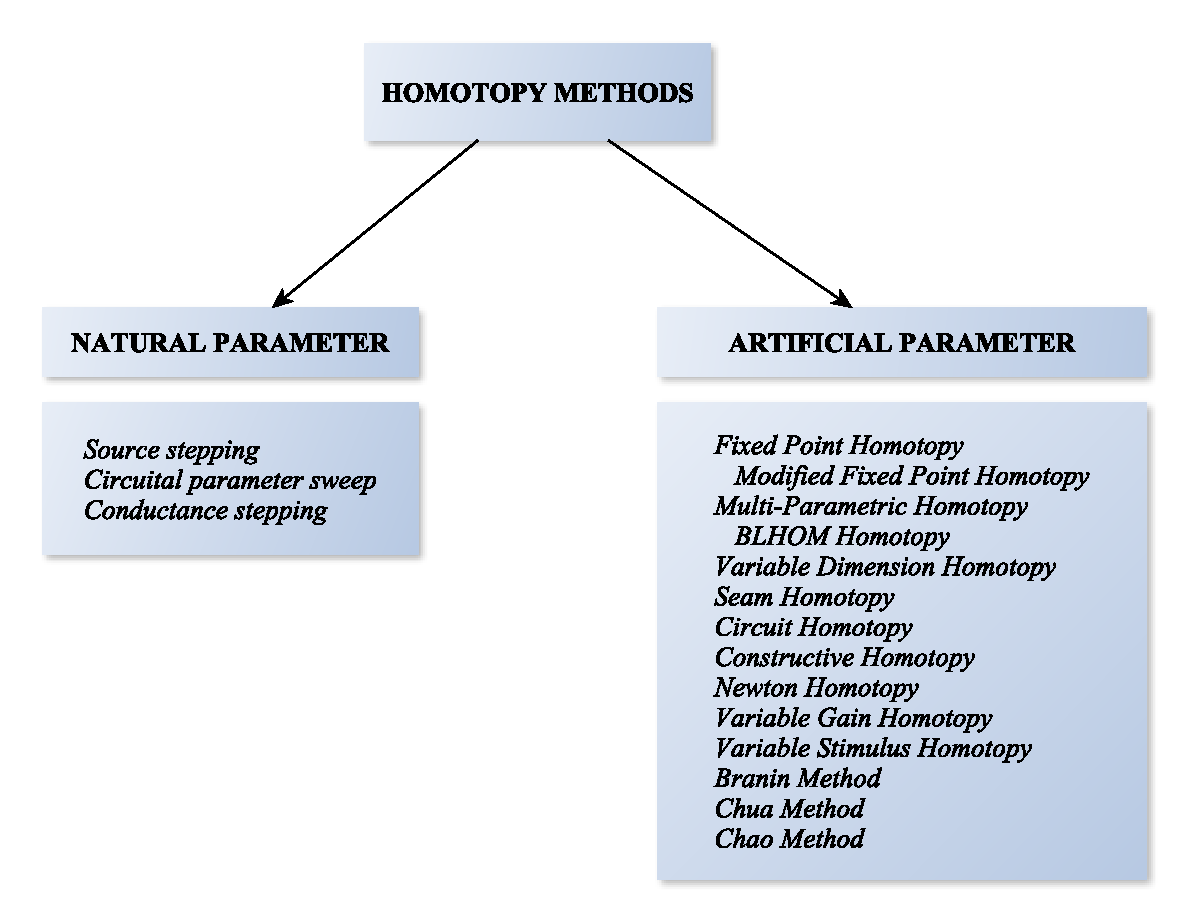
\includegraphics[width=14cm]{figs/homotopy_clas.eps}
\caption{Homotopy classification.}
\label{construc}
\end{figure*}

Double bounded Homotopy is an artificial parameter Homotopy since it adds an extra parameter to the equation system of the circuit, it does not have any direct relationship with the circuit variables.

\section{Multiple operating points}

To establish the equilibrium equation for the circuit is necessary to apply a method like the modified nodal analysis (MNA \cite{stat_1,mnaxx}). Then, it will be possible to formulate the equilibrium equation:

\begin{displaymath}
\pig{f}(\pig{x})=\pig{0}
\end{displaymath}

where $\pig{x}$ represents the unknown vectors for voltage and currents of the circuit.

Being the equilibrium equation a system of simultaneous non-linear equations, these could have: one solution, multiple solutions, or does not have any solution. Nevertheless, the foregoing does not mean much unless defined within the electronic circuits context. Therefore, each case is explained as follows: 

\begin{itemize}
\item {\bf One solution}. One solution means that the circuit has just one operating point. In other words, no matter initial conditions, when the circuit is switched-on it always will settle on the same DC operating point.
\item {\bf Multiple solutions}.The circuit has more than one operating point. Hence, depending on the initial conditions when the circuit is switched-on, it will be established at different operating points. This situation will cause different: nodal voltages and branch currents. 
\item {\bf No solution}. It means that the circuit is operating in a non-valid region for the models employed (MOS, BJT, diodes, among others) in the circuit. Therefore, the absence for a real solution could be just a mathematical result disconnected of the physical reality that rules the circuit.
\end{itemize}

The operating point in an electronic circuit establishes the small signal parameters, those indicate the behavior on amplification, frequency response, noise response, etc. Hence, varying the operating point its qualitative and quantitative behaviors of the circuit are changed. This means that it would be catastrophic for the circuit performance to be established at an operating point unknown to the developer.

Existence of multiple operating points depends of several factors, those will be discussed:

\begin{itemize}
\item Circuit topology could influence the existence of multiple solutions. In \cite{netwth_ns80} established a circuit that contains bipolar transistors, linear and positive resistors, and independent voltage and current sources that has just one operating point. This will remain true as long as it does not contain a positive feedback structure embedded in the topology .
\item Model parameters play a significant role on the multiple point operating point existence, this situation will be combined when positive feedback structures are employed \cite{netwth_lasr}. 
\item The use of non-linear devices whose characteristic curves ($i-v$) have more than one sign change for their derivative (for example: tunnel diode) may cause the existence of multiple operating points\cite{netwth_lasr}.
\end{itemize}

The problem with DC analysis is so complex that even now it is not possible to know for certain when a given circuit has multiple solutions. Also, the Newton-Raphson method (which industrial class simulators employ to find the operating point) is unable to locate more than one solution. Therefore, one way the designer will know the number of operating points the circuit possess is by means of Homotpy methods, these are capable to locate multiple solutions. Besides, there is another reason to use Homotopy methods based on a Newton-Raphson (NR) weakness, that is, NR is a local convergence method. Local convergence means that if initial point is not located close to the operating point, it could diverge to infinity or oscillate and never find the solution. This is a well known situation for circuit designers which are forced "{\it to play}" with different starting points or change other parameters within the Newton-Raphson method to reach convergence of the method to an operating point. Nevertheless, Homotopy has better probability to converge to the solution from any initial point, in fact exist some Homotopy of global convergence or probability one\cite{homo_zeroes,homo_coercitivo}, it means that convergence is guaranteed for one point at least given any starting point.


\section{Homotopy}

Homotopy is capable to find multiple solutions, but the ability to find all the solutions depends on the kind of Homotopy, the selected numerical continuation technique \cite{homo_iberchip03}, and on the type of non-linear circuit. The Homotopy path is formed by the solution family of the Homotopy function, which is formulated as follows:

\begin{equation}
\pig{H}(\pig{f}(\pig{x}),\lambda )=\pig{0}
\label{homotopia}
\end{equation}

where  $\pig{f}(\pig{x})$ is the equilibrium equation for the circuit and $\lambda$ is the continuation parameter. 

The Homotopy path is the solution set of $\pig{H}^{-1}(\pig{0})$, that is a continuous curve that can be traced by some numerical continuation technique or path following method.

\subsection{Homotopy disadvantages}

In order to find multiple solutions all the steps for the numerical continuation method \cite{homo_iberchip03,homo_allgower,homo_allgower2} must continue until the root at  $\lambda=1$ is located.

Nevertheless, the tracing technique continues its route for values $\lambda>1$ up to a turning point and then returns back to $\lambda=1$ finding the next solution (just in case if another solution exist); in figure \ref{procri} a Homotopy path is shown that locates the following solutions at $x^{*}_1$, $x^{*}_2$, $x^{*}_3$ y $x^{*}_4$ . However, after crossing the root $x^{*}_4$ the path continues indefinitely as apparently there are no more solution that produce crossings at $\lambda=1$. Nevertheless, it is not possible to know beforehand the number of solutions for non-linear circuits. Therefore, the trace for the Homotopy path is stopped after an arbitrary number of iterations is reached; this technique is empirical, inefficient, and does not ensure that more solutions exist after tracing is stopped.

\begin{figure}[hbtp]
\psfrag{L}{$\lambda$}
\centering
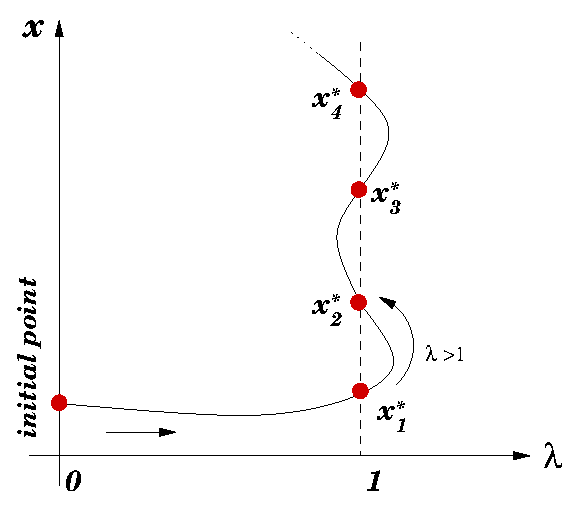
\includegraphics[width=7cm]{figs/tray.eps}
\caption{Stop criterion problem.}
\label{procri}
\end{figure}

The Homotopy method takes more computing time to locate the same operating point than the NR method, given the same initial point. This is the result of the fact that the convergence rate of the NR method is quadratic while the convergence rate of the Homotopy method is linear. Hence, strategies should be implemented in order to reduce the computing time for Homotopy. One possible strategy is to design a stop criterion \cite{homo_iscas05} for Homotopy, which guarantees that no more solutions exist in the selected path.


\section{Double solution line Homotopy}

On the traditional Homotopy \cite{homo_ArtificialP,homo_yamamura} initial operating points are located at $\lambda=1$ because its value is normalized. Nevertheless, $\lambda$ can be chosen any value as the point where the crossing through the operating points takes place.

Therefore, it is possible to establish the following:

\begin{Theod}
{\bf Solution line}
\begin{displaymath}
\lambda-a=0
\end{displaymath}

where $\lambda$ is the Homotopy parameter and $a$ is the value of $\lambda$ where the equilibrium equation solution is located. The value of $\lambda=a$ replaces the value of $\lambda=1$ as the depiction of the imaginary line where solutions of $f(x)$ are located.

\label{InestCond1}
\end{Theod}

An example of traditional Homotopy is Newton's Homotopy, which counts with the solution line at $\lambda=1$. The formulation is as follows:     

\begin{equation}
\pig{H}(\pig{f}(\pig{x}),\lambda ) =
\pig{f}(\pig{x})-(1-{\lambda})\pig{f}(\pig{x}_{0}) = 0
\label{lineasolH1}
\end{equation}

where $f(x)$ is the equilibrium equation, $x_0$ is the initial point of the Homotopy, and $\lambda$ is the Homtopic parameter.

Now, Newton's Homotopy is formulated to have as the solution line the value of $\lambda=a$.

\begin{equation}
\pig{H}(\pig{f}(\pig{x}),\lambda ) =
a\pig{f}(\pig{x})-(a-{\lambda})\pig{f}(\pig{x}_{0}) = 0
\label{lineasolH}
\end{equation}

where $f(x)$ is the equilibrium equation for the circuit,  $x_0$ is the initial point of the Homotopy, and $\lambda$ is the Homotopy parameter. This version of Newton's Homotopy is capable to locate on the solution line $\lambda=a$.

In figure \ref{fig:subfig:sol} is shown, in general way, the aspect of a Homotopy path with solution line at $\lambda=a$. This path is the same (in scale) to the path shown in figure \ref{procri} with the fundamental difference that solution line is not obligatorily located $\lambda=1$. Figure \ref{fig:subfig:sol3} shows how each solution is found after the trajectory crosses through a turning point so the resulting path will tend to be located in the surrounding region of the solutions, which now will be called {\it region of solutions}.

At this moment, the {\it region of solutions} contains the operating points and the return points, but does not include neither the initial point nor final point of the path, which could be interesting since it would mean that the Homotopy path is entirely bounded inside such region. The existence of a second solution line would cause the Homotopy path to transform with purpose to keep its unity and, simultaneously, crossing through both solution lines.

\begin{figure}[hbtp]
\begin{center}
%% --- start of first subfigure ---
\subfloat[Solution line]{
	\label{fig:subfig:sol}
	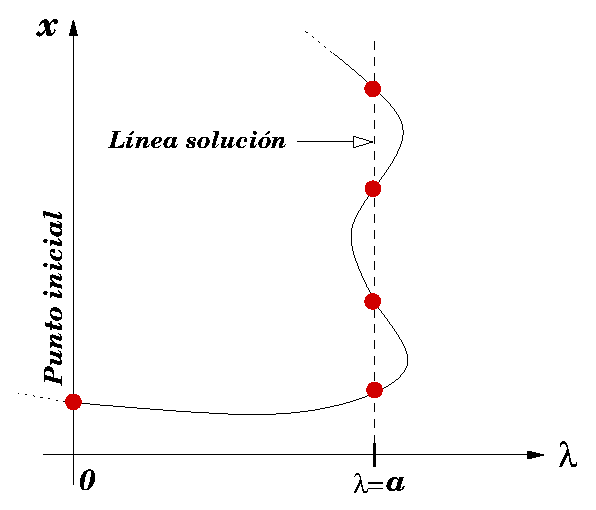
\includegraphics[scale=0.75]{figs/chap3/figs/sol.eps}}
\hspace{-0.025in}
%% --- start of second subfigure ---
\subfloat[Delimitation region for the Homotopy path]{
	\label{fig:subfig:sol3}
	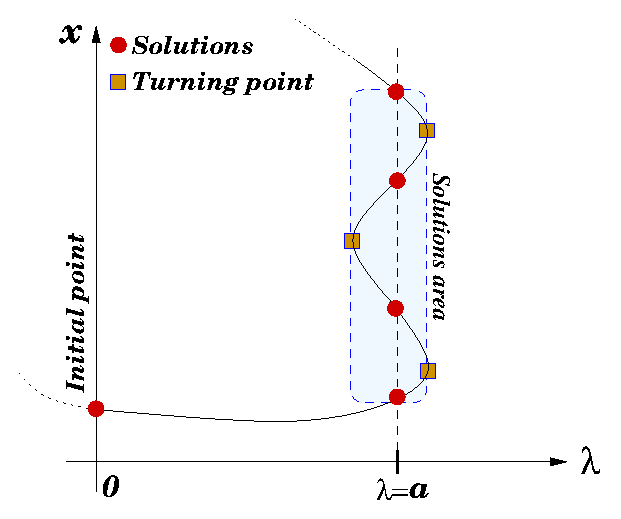
\includegraphics[scale=0.75]{figs/chap3/figs/sol3.eps}}
\end{center}
\caption{Region of solutions.}
\label{fig:subfig}
\end{figure}

Under the condition of existence of two solution lines, one located at $\lambda=a$ and the other at $\lambda=b$, the Homotopy formulation is:

\begin{equation}
\pig{H}(\pig{f}(\pig{x}),\lambda ) =\pig{0}
\label{H2M}
\end{equation}

where $\lambda$ is the Homotopy variable and $\pig{H}^{-1}(\pig{0})$ the family of solutions that forms the Homotopy path, so:

\begin{itemize}
\item For $\lambda=0.5(a+b)$ the solution of $H^{-1}(.)$ is known or easy to obtain using computers. This point is known as Homotopy's initial point ($\lambda_i$).
\item For $\lambda=a$, $\pig{H}(\pig{f}(\pig{x}),\pig{a} )=\pig{f}(\pig{x})$. Means that at $\lambda=a$ all the solutions for $\pig{f}(\pig{x})$ are located.
\item For $\lambda=b$, $\pig{H}(\pig{f}(\pig{x}),\pig{b} )=\pig{f}(\pig{x})$. This means that at $\lambda=b$ all the solutions for $\pig{f}(\pig{x})$ are located.
\item The path for $\pig{H}^{-1}(\pig{0})$ is a continuous function of $\lambda$ within the range of $a \leq \lambda \leq b $. 
\end{itemize}

That said, the Homotopy function for double line of solution can be reformulated as follows:

\begin{displaymath}
\pig{H}(\pig{f}(\pig{x}),\lambda ) = \left\{\begin{array}{ll}
f(x^*)=0 & \textrm{para $\lambda=a$ y $x=x^*$}\\
f(x^*)=0 & \textrm{para $\lambda=b$ y $x=x^*$}
\end{array}\right.
\end{displaymath}

where $\lambda=a$ and $\lambda=b$ are the solution lines, and $x^*$ is any solution for $f(x)$. This means that for each solution line the root are repeated.

The double line of solution extends the concept of solution line:

\begin{Theod}
{\bf Double solution line}
\begin{displaymath}
%\shadowbox{
\begin{tabular}{l}
$\lambda-a=0$ \\
$\lambda-b=0$ \\
\end{tabular}
%}
\end{displaymath}

where $\lambda$ is the Homotopy parameter, $a$ and $b$ are the values of $\lambda$. The Homotopy function is the same as the original equation system.

\label{InestCond2}
\end{Theod}

The result is a continuous curve between the Homotopy's initial point $\lambda_i$ and the desired solution (at $\lambda=a$ or $\lambda=b$). In figure \ref{fig:subfig1:Y1} is outlined the behavior of the Homotopy path for an uneven number of solutions. The area between both solution lines ($a \leq \lambda \leq b $) will be named internal region. The initial point $A$ of the path lies in between the two lines of solution. The Homotopy path cross through the solutions (each line of solution) returning as many times as solutions exist ($S1,S2$, and $S3$), nevertheless, after crossing the last solution ($S3$) the path will not return because there are no more solutions, but will continue the route indefinitely outside the internal region. Finally, in that figure is shown how the solution regions are attached to form one single region that includes the solutions at $\lambda=a$, $\lambda=b$, and the initial point $A$; that means greater delimitation of the path

\begin{figure}[hbtp]
\psfrag{i}{$a \leq \lambda \leq b $}
\psfrag{o}{$\lambda$}
\begin{center}
%% --- start of first subfigure ---
\subfloat[Path for an uneven number of solutions]{
	\label{fig:subfig1:Y1}
	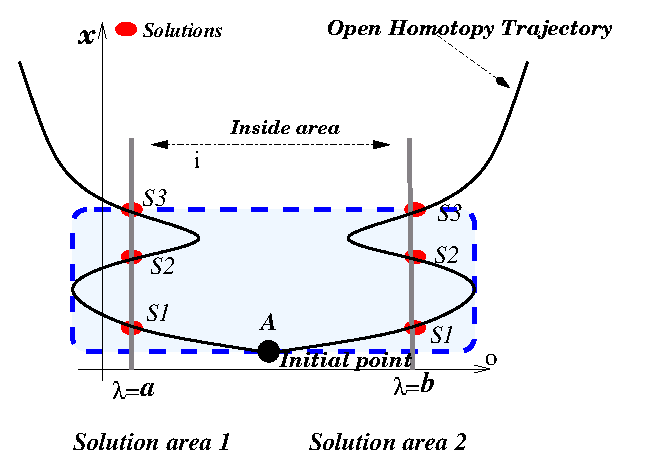
\includegraphics[scale=0.73]{figs/chap3/figs/solsimpar.eps}}
\hspace{-0.025in}
%% --- start of second subfigure ---
\subfloat[Path for an even number of solutions]{
	\label{fig:subfig1:Y2}
	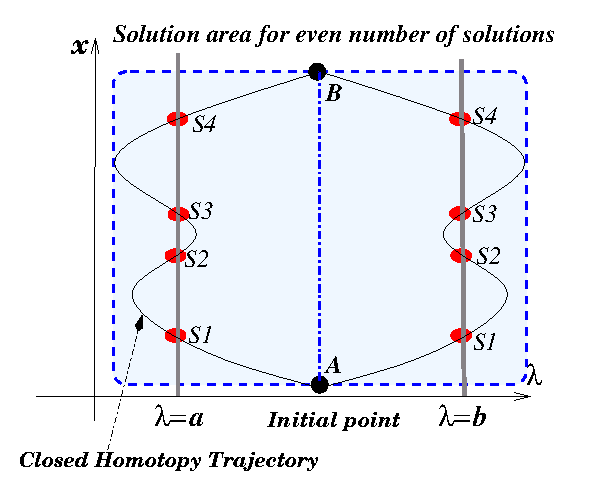
\includegraphics[scale=0.73]{figs/chap3/figs/solspar.eps}}
\end{center}
\caption{Solution paths.}
\label{fig:subfig1}
\end{figure}

The behavior of the path is now analyzed when an even number of solutions exist, particularizing with the case of four solutions. Figure \ref{fig:subfig1:Y2} shows a double line of solution Homotopy for an equation with four solutions. The path starts at $A$, from this point the path cross through solution $S1$ leaving the intermediate region toward the solution lines $a \leq \lambda \leq b $. Afterwards, when crossing through the second solution the path returns to the intermediate region and so on until the last solution ($S4$). Given that the equation to be solved has an even number of solutions, the path ends up inside the {\it intermediate region} reaching the final point $B$. Finally, both lines of solution attach their solution regions covering the initial point $A$, the final point $B$, turning points , and operating points. This new region of solutions denoted by the shaded region can be drawn including a stop strategy, as tracing just half of the path from $A$ to $B$ through $\lambda=a$ or $\lambda=b$ is enough to know the rest of the path. Nevertheless, when the number of solutions is uneven, the Homotopy path does not close, therefore is not possible to establish a general stop criterion.

In figure \ref{fig:subfig1:Y2} there is a straight line (dash-dot) joining points $A$ and $B$, which split the Homotopy path in two symmetrical branches that will be named: symmetry axe. From this axe, the Homotopy path behaves symmetrically (like a mirror), which is valid for an even or uneven number of solutions. The definition for the symmetry axe is given by:

\begin{Theod}
In a Homotopy system with double line of solution, the {\bf symmetry axe} is:
\begin{displaymath}
%\shadowbox{
\lambda=(a+b)/2
%}
\end{displaymath}

where $\lambda$ is the Homotopy parameter, $a$ and $b$ define values for each line of solution.
\label{InestCondh2}
\end{Theod}

\section{Double bounded Homotopy}

On the previous section it was shown that it is not possible to find a stop criterion for an uneven number of solutions. Therefore, in order to solve this problem, the equilibrium equation $f(x)$ is squared, duplicating the number of roots, creating this way an even number of them and closing the path as a consequence. First, figure \ref{Z1}(a) shows the Homotopy path for an equilibrium  equation with two solutions (even number of solutions). Second, figure \ref{Z1}(b) shows the Homotopy path for an equilibrium equation with three solutions (uneven number of solutions). The qualitative characteristics of this new Homotopy path can be enumerated as follows (see figure \ref{Z1}):

\begin{enumerate}
\item  Path is closed for an even or uneven number of solutions.
\item  Path does not cross solution lines. Solution occurs when path touches obliquely the solution line.
\item  Symmetry axis. The Homotopy path (reflected branch) for each solution line starts and ends in the symmetry axis creating a closed path.
\item  Solution regions is bounded by both solution lines ($\lambda=a$ and $\lambda=b$), initial point $A$, and final point $B$.
\end{enumerate}

\begin{figure}[hbtp]
\psfrag{o}{$\lambda$}
\centering
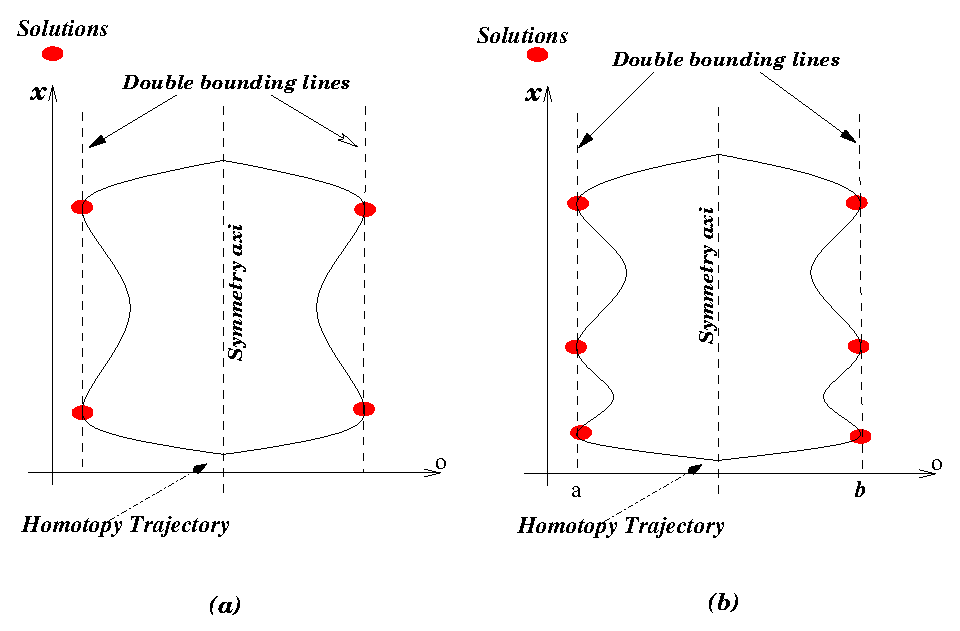
\includegraphics[scale=0.95]{figs/chap3/figs/ddb.eps}
\caption{(a) Even number of solutions (b) Uneven number of solutions}
\label{Z1}
\end{figure}

On one hand, the path is closed and symmetrical, on the other hand, tha path touch obliquely the solution lines in an effect to be called {\it rebound}. The result is that this {\it rebound} effect of the Homotopy path cause to close it no matter the number of solutions (even or uneven).

The previous definitions describe in a general way a new kind of Homotopy named double bounded Homotopy. This new Homotopy adds one restriction to the Homotopy equation \ref{homotopia}, which shows that $\lambda\in \Re $ is only for $a \le\lambda\le b$. Next, a Homotopy of this kind is described.

\subsection{Double bounded Homotopy}

The double bounded Homotopy \cite{homo_iscas05} is defined by:

\begin{equation}
H(f(x),\lambda)=CQ+e^Q\ln(Df^2(x)+1)
\label{fx1}
\end{equation}

where $f(x)$ is the function to be solved, $\lambda$ is the Homotopy parameter, $C$ and $D$ are positive constants of the Homotopy, and $Q$ is given by:

\begin{displaymath}
Q=(\lambda-a)(\lambda-b)
\end{displaymath}

where $a$ and $b$ are values for the double bounding line.

The term $(Df^2(x)+1)$ is employed to guarantee that the argument of the logarithmic function does not become negative. The logarithmic term is used to soften the big values from the square of $f(x)$. Nevertheless, it is also possible formulate the Homotopy function as:

\begin{equation}
H(f(x),\lambda)=CQ+De^Q f^2(x)
\label{fx22}
\end{equation}

Both Homotopies are on essentially the same, except that Homotopy from equation \ref{fx1} is employed with circuits influenced by components having exponential branch functions, while the Homotopy from equation \ref{fx22} can be used with any kind of function.

In figure \ref{halftrack} can be seen how the Homotopy path starts at $A$ over the symmetry axis and finishes when detects that path has crossed the symmetry axis again at $B$, meaning that the path on a symmetric branch has been completed meeting the stop criterion.

\begin{displaymath}
\begin{array}{l}
A=(x_i,(a+b)/2)\\
B=(x_f,(a+b)/2)
\end{array}
\end{displaymath}

\begin{figure}[hbtp]
%\psfrag{xi}{{\small $P_i$}}
%\psfrag{xf}{{\small $P_f$}}
\psfrag{o}{$\lambda$}
\centering
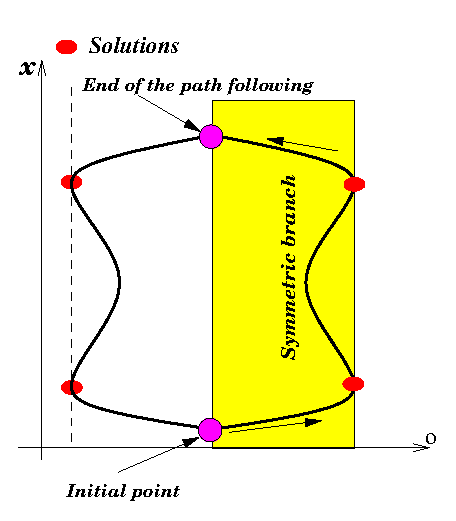
\includegraphics[width=7cm]{figs/chap3/figs/dbh2.eps}
\caption{Stop criterion.}
\label{halftrack}
\end{figure}

The properties for this new Homotopy are presented on the following sub-sections:

\subsubsection{Lambert $\cal W$ function}

Lambert $\cal W$ function is a transcendental function that plays a very important role proving the properties for the double bounded Homotopy. In 1798 mathematician Lamber laid the foundations of the Lambert $W$ function. Later, Euler completed the work characterizing in more detail this function and using the letter $\cal W$ to call it. For more than a century it was used for different mathematical problems, all of them using their unique notation, it was in \cite{homo_onlambert} that the name was formalized and its properties gathered.

The main property \cite{homo_onlambert}, \cite{homo_lambertsec}, \cite{homo_lambertmaple} of the Lambert $\cal W$ function is given by:

\begin{equation}
\begin{array}{l}
{\cal W}(z)e^{{\cal W}(z)} = z
\end{array}
\label{W1}
\end{equation}

where $z$ is a function.

This function, basically, has been used on the mathematical field \cite{homo_onlambert},  physics \cite{homo_wfisica} and electronics \cite{homo_banwell}\cite{homo_banwell2}. This function is fundamental to explain the properties of the double bounded Homotopy.

\subsubsection{Symmetry in Homotopy}

The characteristics of the Double Bounded Homotopy can be shown using algebraic analysis of the equation \ref{fx1} supported by the use of the Lambert $\cal W$ function.

First, equation (\ref{fx1}) can be represented as follows:

\begin{displaymath}
\begin{tabular}{c}
$-Qe^{-Q}=\frac{\ln(Df^2(x)+1)}{C}$ \\
\end{tabular}
\label{y1}
\end{displaymath}

Now, after replacing $-Q={\cal W}(z)$, is obtained:

\begin{displaymath}
\begin{tabular}{c}
${\cal W}(z) e^{{\cal W}(z)}=\frac{\ln(Df^2(x)+1)}{C}$\\
\end{tabular}
\label{y2}
\end{displaymath}

Therefore, solving for $z$, the result is:

\begin{displaymath}
\begin{tabular}{c}
$z=\frac{\ln(Df^2(x)+1)}{C}$\\
\end{tabular}
\label{y3}
\end{displaymath}

Then, $Q$ becomes:
\begin{equation}
Q=-{\cal W}(\frac{\ln(Df^2(x)+1)}{C})
\label{y3b1}
\end{equation}

Where $Q$ represents the double bounding given by:
\begin{displaymath}
Q=(\lambda-a)(\lambda-b)
\end{displaymath}

Replacing this expression in equation (\ref{y3b1}) this expression is obtained:

\begin{displaymath}
(\lambda-a)(\lambda-b)=-{\cal W}(\frac{\ln(Df^2(x)+1)}{C})
\label{y4}
\end{displaymath}

This equation is solved for $\lambda$. The result are two symmetrical branches:

{
\begin{equation}
\begin{array}{l}
\lambda_1(\pig{x})=0.5(a+b)+0.5\sqrt{(b-a)^2-4{\cal{W}}(\ln(Df^2(\pig{x})+1)/C)} \\ \\
\lambda_2(\pig{x})=0.5(a+b)-0.5\sqrt{(b-a)^2-4{\cal{W}}(\ln(Df^2(\pig{x})+1)/C)}
\end{array}
\label{ramass}
\end{equation}
}

Branches $\lambda_1(\pig{x})$ y $\lambda_2(\pig{x})$ represent the reflexed branches of the Homotopy path seen from the symmetry axis. The analysis of these expressions leads to determine the following properties:

\begin{itemize}
\item {\bf Narrowing.} The range of values for $\lambda_1(\pig{x})$ and $\lambda_2(\pig{x})$ are:
\begin{displaymath}
\begin{array}{l}
0.5(a+b) \leqslant \lambda_1(\pig{x}) \leqslant b\\\\
\hspace{13mm}a \leqslant \lambda_2(\pig{x}) \leqslant 0.5(a+b)
\end{array}
\end{displaymath}

This range narrows the excursion of the Homotopy path as shown in figure \ref{halftrack}.

\item {\bf Symmetry axis.} From the range of values for $\lambda_1(\pig{x})$ and $\lambda_2(\pig{x})$, can be concluded that the matching point between the reflexed branches is the symmetry axis:

\begin{displaymath}
\lambda_{sym}=(a+b)/2
\end{displaymath}

In equation \ref{ramass} it can be seen each of the two branches for the Homotopy path. Next, it be demonstrated the existence of a symmetry for the Homotopy path.

As shown in figure \ref{simetria}, this relationship must be satisfied:

\begin{displaymath}
\lambda_1(x)-\lambda_{sym}=\lambda_{sym} -\lambda_2(x)
\end{displaymath}

Replacing the value of $\lambda_{sym}$, we obtain:

\begin{displaymath}
\lambda_1(x)-0.5(a+b)=0.5(a+b)-\lambda_2(x)
\end{displaymath}

Also, replacing the value of $\lambda_1$ and $\lambda_2$ for their respective functions yields the following relationship:

\begin{displaymath}
\begin{array}{l}
0.5(a+b)+0.5\sqrt{G(\pig{x})}-0.5(a+b)= \\ \\
0.5(a+b)-0.5(a+b)+0.5\sqrt{G(\pig{x})}
\end{array}
\end{displaymath}
donde
{\small $G(\pig{x})=(b-a)^2-4{\cal{W}}(\ln(Df^2(\pig{x})+1)/C)$}.

Eliminating terms it follows that:
\begin{displaymath}
\begin{array}{c}
0.5\sqrt{G(\pig{x})}=0.5\sqrt{G(\pig{x})} \\
0=0
\end{array}
\end{displaymath}

Proving this equality shows that the Homotopy path is symmetrical around the symmetry axis.

{
%\small
\begin{figure}[hbtp]
\psfrag{o}{\tiny $\lambda$}
\psfrag{o1}{\tiny $\lambda_1(x)$}
\psfrag{o2}{\tiny $\lambda_2(x)$}
\psfrag{o3}{\tiny $\lambda_1(x)-\lambda_{sym}$}
\psfrag{o4}{\tiny $\lambda_{sym}-\lambda_2(x)$}
\centering
\includegraphics[scale=1]{figs/simetria.eps}
\caption{Symmetry axi of the homotopic path}
\label{simetria}
\end{figure}
}

\item {\bf Initial point $A=(x_i,\lambda_i)$}. The point where the Homotopy path starts is placed right in the symmetry axis, therefore $\lambda_i=(a+b)/2$. Hence, replacing $\lambda_i$ in equation \ref{fx1} and solving for $C$:

{
\small
\begin{displaymath}
\begin{array}{c}
C=4\,{\frac {{{\rm e}^{-1/4\, \left( a-b \right) ^{2}}}\ln  \left(
 D {{\it f(x_i)}}^{2}+1 \right) }{ \left( a-b \right) ^{2}
}} \\\\
\end{array}
\end{displaymath}
}

Once the point $x_i$ is chosen (arbitrary) it is possible to find the value for $C$ and $D$ to validate the previous equation. The easiest way is to pick a fixed value for $D$ and define the value for $C$ using the previous formula. In the same way, if choosing the initial point decide the values for $C$ and $D$, it is possible to see the problem just the other way around and infer that if values for $C$ and $D$ are established, they will modify the initial point. Therefore, the Homotopy path is strongly influenced by values $C$ and $D$. To study the effect of $C$ and $D$ on the initial point, first $\lambda=(a+b)/2$ is replaced in the Homotopy equation, giving as result:

\begin{displaymath}
\begin{array}{c}
C(-a/2+b/2)(a/2-b/2)+e^{(-a/2+b/2)(a/2-b/2)}ln(D[f(x)]^2+1)=0
\end{array}
\end{displaymath}

This places the path in the symmetry axis and, therefore, at the initial point. Now, solving $f(x)$ it gives:

\begin{equation}
%\shadowbox{
%$
f(x_i)=\pm {{\sqrt{ D(e^{\big ( {{C(a-b)e^{(a-b)^2/4} }  \over { 4   }} \big ) }-1 )}} \over {D}}
%$}
\label{formulaxi}
\end{equation}

This expression shows the effect of $C$ and $D$ on the initial point ($x_i$). $D$ may contain small values, but not zero given the fact that at this point the expression is undefined. Now, another particular case about the effects of $C$ and $D$ over certain $f(x)$ is presented.

The function is:
\begin{displaymath}
f(x)=x-10
\end{displaymath}

Now, replacing the previous equation into equation \ref{formulaxi}.
\begin{displaymath}
x-10=-(D(e^{0.321C}-1))^{1/2}/D
\end{displaymath}

In figure \ref{cydx1} can be seen the complete dot plane for the initial points with respect to $C$ and $D$. The initial point grows exponentially compared to $C$ and $D$, except that grows faster with respect to $C$. It also shows the behavior of $x_i$ when ${C \over D}=1$, ${C \over D}=2$, ${C \over D}=3$, and $D=1/C$. As the ratio of $C \over D$ increases, the absolute value for the initial point has bigger values. In summary, values for $C$ and $D$ affect the initial point $x_i$ over the symmetry axis. This also depends of the circuit to be solved, that is, from the equilibrium equation $f(x)$. So, the initial point $x_i$ can be obtained fixing the values for $C$ and $D$ arbitrary, then solving equation \ref{formulaxi} or choosing a value for $x_i$ arbitrary and solving the resultant equation \ref{formulaxi} for $C$ and $D$ (selecting $C$ and $D$ proportionally).

\begin{figure}[hbtp]
\centerline{
\epsfxsize=85mm
\epsffile{chap4/figs/cydx1.eps}}
\caption{Relationship between $C$, $D$, and initial point $x_i$.}
\label{cydx1}
\end{figure}

\item {\bf Circuital interpretation of double bounded Homotopy}.

The circuital interpretation for the double bounded Homotopy can be obtained from the expression for Homotopy at the initial point (symmetry axis), given by equation \ref{formulaxi}. From that equation can be concluded that non-linear current sources are present in the circuit ($K_1$, · · · ,$K_n$) connected at each node of the circuit and non-linear voltage sources ($K_{n+1}$, · · · ,$K_{n+l}$) connected in series to each constant voltage source, where $n$ is the number of nodes and $I$ the number of constant voltage sources ($E$).

\begin{equation}
I_{K_i}= {{\sqrt{ D(e^{\big ( {{C(a-b)e^{(a-b)^2/4} }  \over { 4   }} \big ) }-1 )}} \over {D}}
\label{Ikn}
\end{equation}
donde $i=[1,n]$. 
\begin{equation}
E_{K_j}= {{\sqrt{ D(e^{\big ( {{C(a-b)e^{(a-b)^2/4} }  \over { 4   }} \big ) }-1 )}} \over {D}}
\label{Ikn2}
\end{equation}
donde $j=[n+1,n+l]$.

Finally, the circuital interpretation of the Homotopy at the symmetry axis can be observed in figure \ref{circ1}.


\begin{figure*}[tbp]
\centerline{
\epsfxsize=130mm
\epsffile{figs/circ_1.eps}}
\caption{Circuital interpretation for the double bounded Homotopy.}
\label{circ1}
\end{figure*}

\end{itemize}

\subsubsection{Multiple varaibles}

When Homotopy is applied to a non-linear equation system with multiple variables, generalization is given by:

\begin{displaymath}
\begin{array}{c}
H_1(f_1(x),\lambda)=CQ+e^{Q}\ln(Df_1^2(x)+1) \vspace{5mm} \\
H_2(f_2(x),\lambda)=CQ+e^{Q}\ln(Df_2^2(x)+1)\\
\vdots \\
H_n(f_n(x),\lambda)=CQ+e^{Q}\ln(Df_n^2(x)+1)\\
\end{array}
\end{displaymath}

where $n$ is the number of equations for $\pig{f}(\pig{x})$, $f_i$ represents each one of the nodel equations and $Q=(\lambda-a)(\lambda-b)$.

\subsubsection{Curved radius}

The curved radius of the Homotopy path will be used as a tool to analyze qualitatively the path behavior in strategic points like solutions and turning points (see figure \ref{radio1}). The curved radius for a curve at a point is the radius for the circle with an equivalent curvature at that point in the curve.

The equation for the curved radius is:

\begin{displaymath}
\rho=  \Bigg |{{(1 + (y')^2)^{3/2}} \over {y''}} \Bigg |
\end{displaymath}

where $y$ is a function $y(x)$, $y'$ is the first derivative of $y(x)$ with respect to $x$ and $y''$ is the second derivative of $(y)x)$ with respect to $x$. In terms of the Homotopy path, the first derivative $y'$ equals to ${ {d \lambda} \over {dx}}$ and the second derivative $y''$ equals to ${ {d^2 \lambda} \over {dx^2}}$.

\begin{figure}[hbtp]
\psfrag{l}{$\lambda$}
\psfrag{z}{$\rho_s$}
\psfrag{v}{$\rho_r$}
\centering
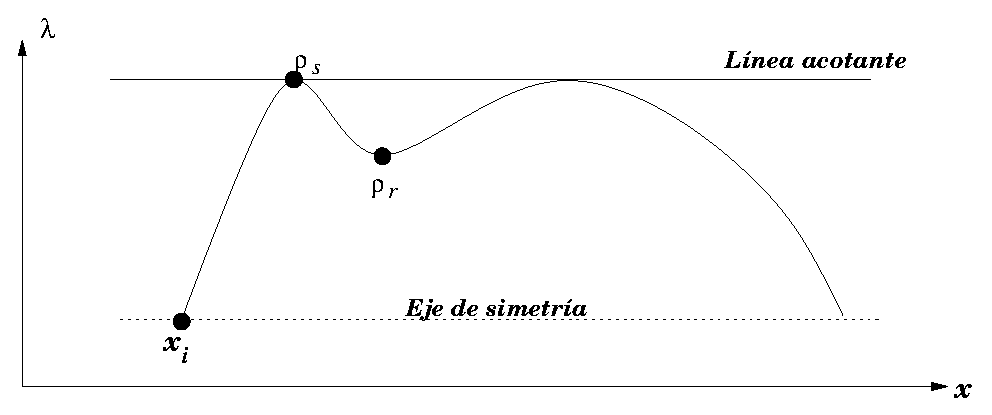
\includegraphics[width=8cm]{figs/chap3/figs/radiob.eps}
\caption{Solution point $\rho_s$ and turning point $\rho_r$}
\label{radio1}
\end{figure}

The slope of the Homotopy path on the solution points and turning points is zero ($y'={ {d \lambda} \over {dx}} =0$), property that can be used to simplify the expression for the curved radius at those points, as:

\begin{displaymath}
\rho= \Bigg | {1 \over {{ {d^2 \lambda} \over {dx^2}}}} \Bigg |
\end{displaymath}

Now, $\lambda$ is derived twice (from equation \ref{ramass} ) with respect to $x$, considering $a$, $b$, $C$ y $D$ as constants. After the derivatives, $f(x)$ is replaced by zero since this is the solution point, it results on the following:

\begin{displaymath}
\rho_{s}= \Bigg | {C(b-a) \over 2D\big [{df(x) \over dx} \big |_{x_s} \big ]^2}\Bigg |
\end{displaymath}

where $x_s$ is the value of the solution, $a$ and $b$ are values for the solution lines.

The equation $\rho_{s}$ allows to establish that the distance between solution lines affects the sharpen of the Homotopy path on the solutions, in such a way that the curve sharpens as the solution lines get closer (between them) and flattens as the solution lines separate. Besides, the ratio $C \over D$ affects the curve, flattens at the solution when the ratio $C \over D$ increase and sharpens when ratio $C \over D$ decrease.

The point where the path returns to the solution search is called turning point $\rho_r$. The study of the curved radius at the turning point $\rho_r$ is completed with the study of the curved radius at the solutions $\rho_s$ to understand more deeply the qualitative behavior of the Homotopy path. At the turning point the derivative of $\lambda$ with respect to $x$ equals zero. Besides, the turning point matches spatially with the critical points of the function $f(x)$, then the derivative of $f(x)$ with respect to $x$ is zero, also. These two attributes for the turning point help to simplify the curved radius, being expressed as:

{
\small{
\begin{displaymath}
\rho_{r}=\Bigg | {\sqrt{(b-a)^2-4{\cal{W}}({Z \over C})} (f(x)+ {1 \over Df(x)}) (1+{\cal{W}}({Z \over C}))Z \over
2{\cal{W}}({ Z \over C} )  {d^2f(x) \over dx^2}
} \Bigg |_{x_r} \Bigg |
\end{displaymath}}}

{
\small{
\begin{displaymath}
Z=\ln(Df^2(x)+1)
\end{displaymath}}}

where $x_r$ is the value for $x$ at the turning point.

As $f(x)$ is evaluated at $x_r$, produce bigger values, the turning points flatten because the curved radius grows. This depends of the non-linear nature of the equilibrium equation and, therefore, not so simple to predict.

What has been said before in this section indicates that the Homotopy path tends to flatten near the solution lines. Suppose that a Homotopy path have solution lines at $\lambda=0$ and $\lambda=1$. Figure \ref{xxx1}(a) shows the symmetry branch located at the right ($\lambda=1$). This phenomenon is corroborated by means of simulations of several circuits y non-linear equations.

\begin{figure}[hbtp]
\centering
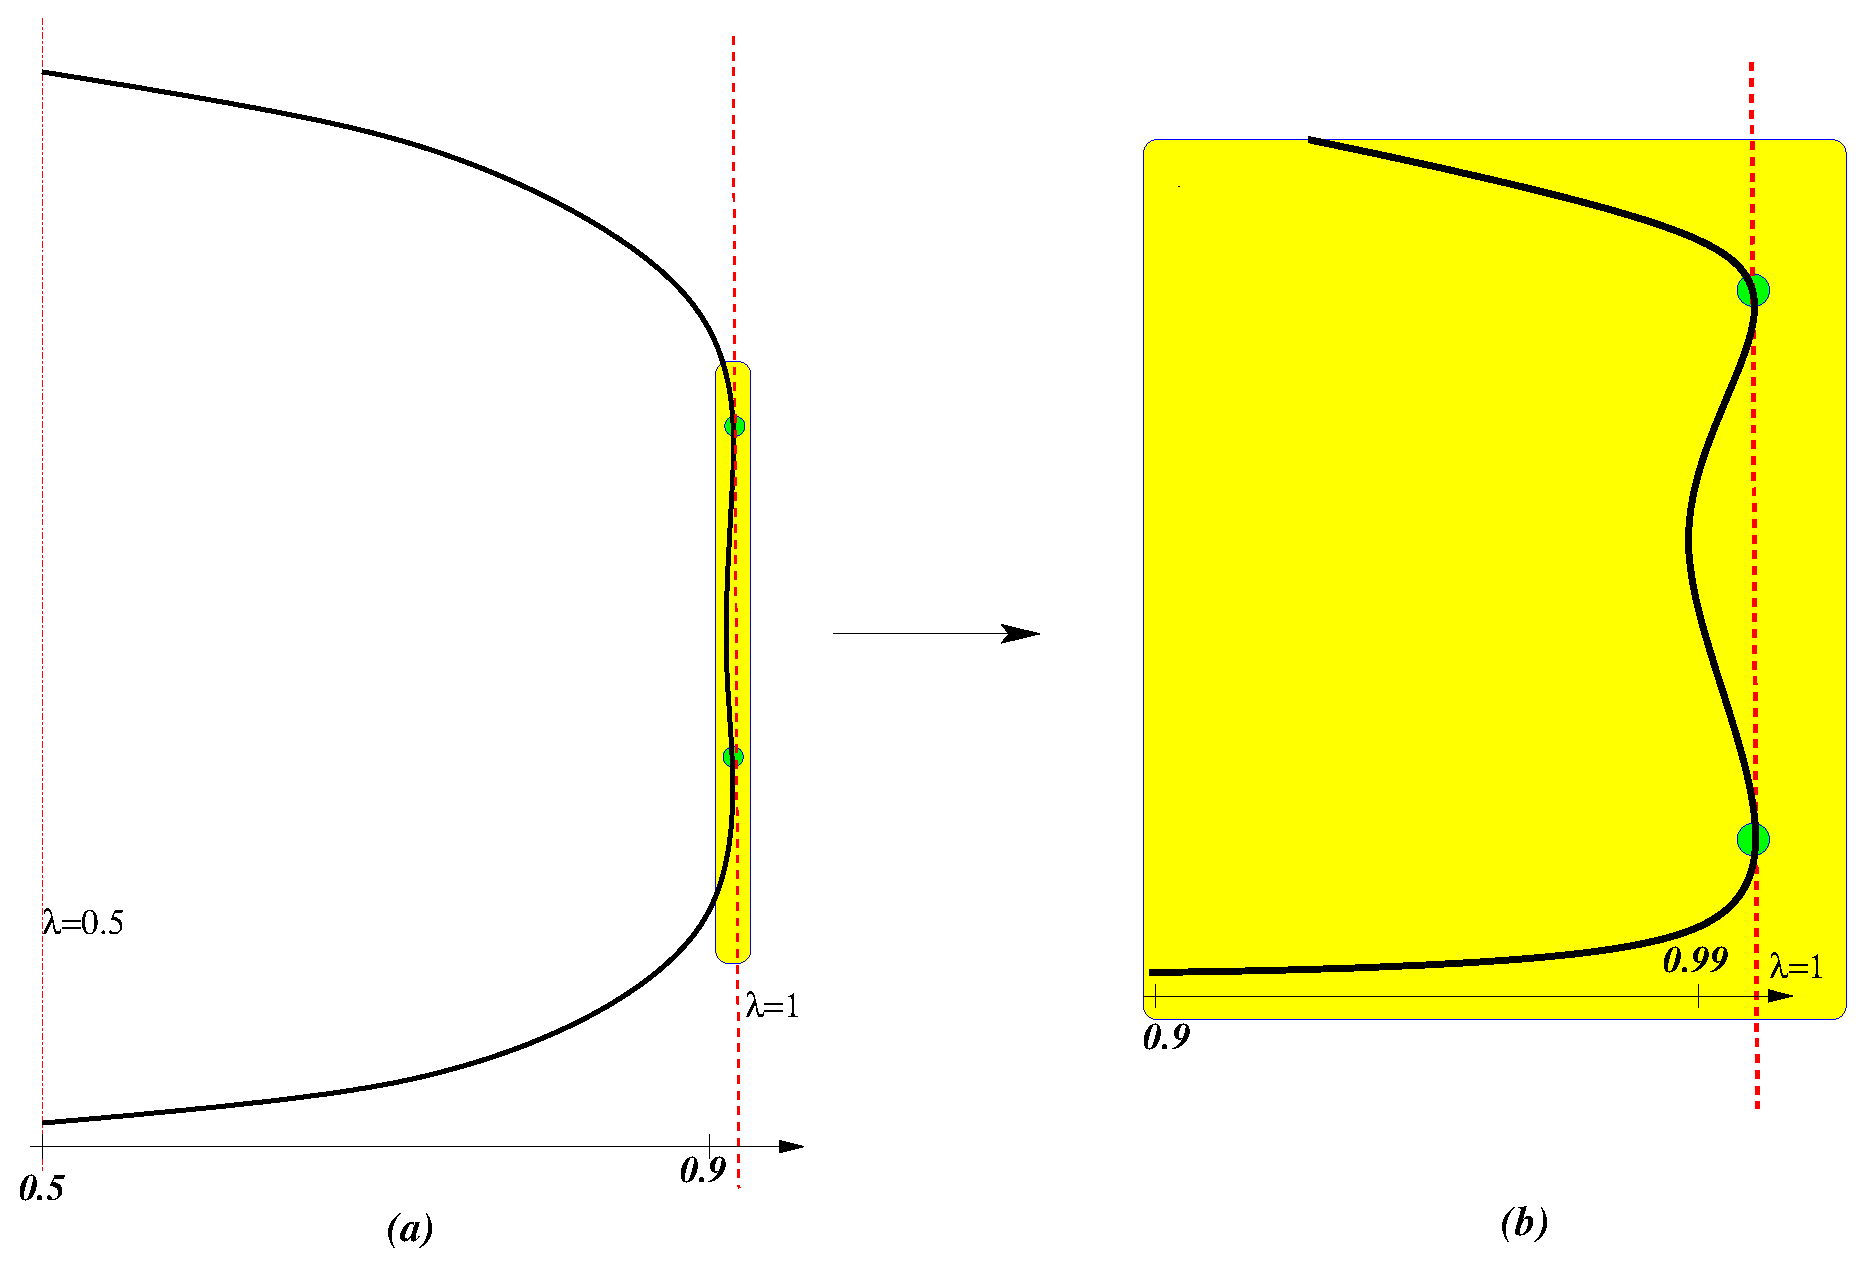
\includegraphics[scale=0.45]{figs/curvatura.eps}
\caption{a) Typical Homotopy path b) Close-up to solution region.}
\label{xxx1}
\end{figure}

\subsubsection{Solution lines}

The behavior of the Homotopy path is affected by the difference $a-b$ and not by the single values for $a$ and $b$. Therefore, the value for $a$ is chosen by convention as $a=0$. Likewise, $b=1$ is chosen by normalization.

\section{General description for the stop criterion}

The proposed scheme has the objective to provide a stop criterion to the Homotopy. It is based on the principle to deform the Homotopy path, until it is encapsulated between two constant narrowing lines ($\lambda=a$ and $\lambda=b$), where each constant line contains its symmetrical branch of the Homotopy path. This path touches obliquely the narrowing solution lines. This means that each line $\lambda=a$ and $\lambda=b$ is never crossed by the Homotopy path. The result is that both symmetric branches form a closed circle between $\lambda=a$ and $\lambda=b$. The diagram in figure \ref{esquemag} shows the proposed  general Homotopy flowing scheme.

\begin{figure*}[tbp]
{\tiny
\centerline{
%\psfrag{l}{$\lambda$}
\centering
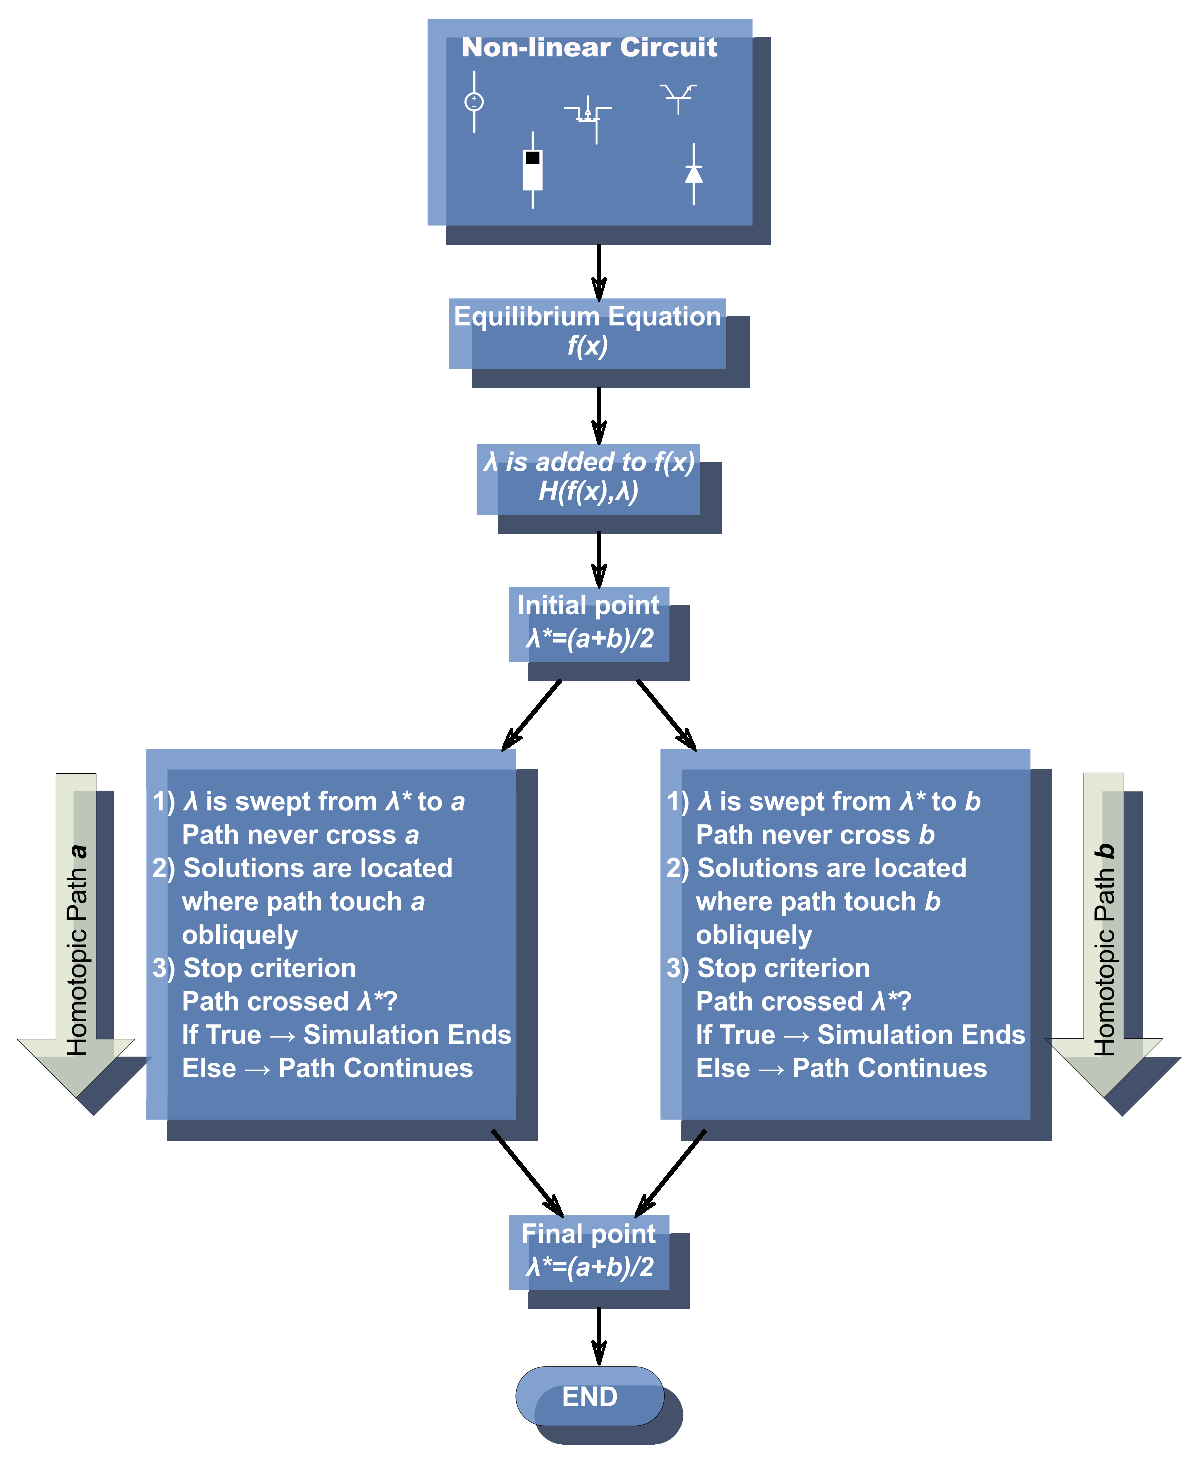
\includegraphics[scale=0.5]{figs/esquema_general_propuesto.eps}}
\caption{Proposed general Homotopy flowing scheme.}
\label{esquemag}}
\end{figure*}

The first step consists in the formulation of the equilibrium equation from the non-linear circuit to be solved. Afterwards, the Homotopy parameter is added to the latter equation. The Homotopy equation is obtained. The next step is to define the initial point midway between  $a$ and $b$ ($\lambda=(a+b)/2$). From the initial point is possible to take two directions, one direction goes to the bounding line $\lambda=a$ and the other direction goes to the bounding line $\lambda=b$. In both cases the same solutions are found. Solutions are detected on each oblique touch of the path with the bounding line ($\lambda=a$ or $\lambda=b$). Finally, when a crossing through the symmetry axis is detected ($\lambda=(a+b)/2$) it can be concluded that one of the symmetry branches has finished its path, this activates the stop criterion considering that the simulation has concluded.

\section{Cases of study}

Double bounded homotopy has been developed to simulate non-linear circuits with multiple solutions. This section will show some Homotopy simulations for different kinds of circuits to expose the proposed new method to a variety of non-linear functions.

\subsection{Non-linear equation system}

In order to explain the use of the Homotopy for a two-dimensional example, Homotopy is applied to the following NAEs:

\begin{displaymath}
\begin{array}{c}
f_1(x_1,x_2)=(x_2-1)(x_2-4)(x_2-6)+x_1=0\\
f_2(x_1,x_2)=(x_1-3)(x_1-6)(x_1-9)+x_2=0
\end{array}
\end{displaymath}

Graphical solution of the system is shown in figure \ref{9sol}.

\begin{figure}[hbtp]
\centerline{
\epsfxsize=80mm
\epsffile{chap3/figs/doblelimit_mul_1.eps}}
\caption{Five solution system.}
\label{9sol}
\end{figure}

The proposed formulation is:

\begin{displaymath}
\begin{array}{c}
H_1(f_1,\lambda)=Q+0.001e^{Q}f_1^2=0\\
H_2(f_2,\lambda)=Q+0.001e^{Q}f_2^2=0\\
\end{array}
\end{displaymath}

where $a=0$ and $b=1$, giving as a result $Q=\lambda(\lambda-1)$.

The initial point for the Homotopy path es given at $x_1 = 2.27896$ and  $x_2 = 0.11622$. Result is shown in figures \ref{homote}, \ref{homote1} y \ref{homote2}.

\begin{figure}[hbtp]
\psfrag{ll}{$\lambda=1.5$}
\psfrag{l}{$\lambda$}
\psfrag{l1}{$\lambda=2$}
\psfrag{x}{$x_1$}
\psfrag{y}{$x_2$}
\centerline{
\epsfxsize=80mm
\epsffile{figs/5sols.eps}}
\caption{Example of Homotopy path for two variables.}
\label{homote}
\end{figure}


\begin{figure}[hbtp]
\psfrag{ll}{$\lambda=1.5$}
\psfrag{l}{$\lambda$}
\psfrag{l1}{$\lambda=2$}
\psfrag{x}{$x_1$}
\psfrag{y}{$x_2$}
\centerline{
%\epsfxsize=80mm
\epsfig{figure=figs/x1lambda.eps, angle=-90,width=0.5\linewidth}}
\caption{$x_1$ against $\lambda$}
\label{homote1}
\end{figure}

\begin{figure}[hbtp]
\psfrag{ll}{$\lambda=1.5$}
\psfrag{l}{$\lambda$}
\psfrag{l1}{$\lambda=2$}
\psfrag{x}{$x_1$}
\psfrag{y}{$x_2$}
\centerline{
%\epsfxsize=80mm
\epsfig{figure=figs/x2lambda.eps,angle=-90,width=0.5\linewidth}}
\caption{$x_2$ against $\lambda$}
\label{homote2}
\end{figure}

\subsection{Circuit with two tunnel diodes}

Tunnel diodes have non-linear behavior, which is shown in Figure \ref{tunelmod}. As it can be seen in the figure, the tunnel diode has three sign changes for the slope. This situation combined with a long load line could produce up to three solutions for the tunnel diode in a circuit. The chosen model for the tunnel chosen for this example contains exponential terms \cite{homo_sze},\cite{homo_shur} and can be expressed as:

\begin{displaymath}
i=I_p({V \over V_p})e^{1-{V \over V_p}}+I_0e^{{q \over {KT}} V}
\end{displaymath}

\begin{figure}[hbtp]
\centerline{
\epsfxsize=65mm
\epsffile{chap4/figs/tunnelmod.eps}
}
\caption{Model for tunnel diode}
\label{tunelmod}
\end{figure}

Exponential terms usually cause numerical overflows, so this circuit represents a challenge for the DBH. Therefore, this example shows a circuit (ERDD) with two tunnel diodes, one voltage source and a resistor in series (figure \ref{2tunel}).

\begin{figure}[hbtp]
\centerline{
\epsfxsize=80mm 
\epsffile{chap4/figs/erdd.eps}
}
\caption{Circuit with two tunnel diodes.}
\label{2tunel}  
\end{figure}

The value for the voltage source $V_1$ is $1V$ and for the resistor $R_2$ is $20\Omega$. Also, both tunnel diodes ($K_3$ y $K_4$) have the same model with coefficients:

$Ip=100 \times 10^{-3}$,
$V_p=50 \times 10^{-3} $, $I_0=1\times 10^{-9}$ y ${q \over {KT}} = 40$. 

The equilibrium equation is formualted from the modified nodal analysis. Also, the system is reduced down to three equations eliminating the nodal voltage $v_1$ because it is constant and equal to the voltage source. Therefore, the system variables for the system are: $I_E$, $v_2$ y $v_3$. Equations are expressed as follows:

\begin{displaymath}
\begin{array}{l}
f_1=  {1 \over 20}-{v_2 \over 20}+I_E =0\\ \\
f_2=  -{1 \over 20}+{v_2 \over 20}+2(v_2-v_3)e^{(1-20v_2+20v_3)} +1\times 10^{-9}e^{(40v_2-40v_3)} =0 \\\\
f_3=  2(v_2-v_3)e^{(1-20v_2+20v_3)}+1\times 10^{-9}e^{(40v_2-40v_3)}-2v_3e^{(1-20v_3)}-1\times 10^{-9} e^{(40v_3)} =0
\end{array}
\end{displaymath}

Now, the DBH is applied to solve the circuit. The Homotopy formulation is expressed this way:

\begin{displaymath}
\begin{array}{c}
H_1(f_1,\lambda)=C\lambda(\lambda-1)+e^{\lambda(\lambda-1)}\ln(Df_1^2+1)=0\\
H_2(f_2,\lambda)=C\lambda(\lambda-1)+e^{\lambda(\lambda-1)}\ln(Df_2^2+1)=0\\
H_3(f_3,\lambda)=C\lambda(\lambda-1)+e^{\lambda(\lambda-1)}\ln(Df_3^2+1)=0\\
\end{array}
\end{displaymath}

where the bounding lines have values $a=0$ and $b=1$, the coefficients of the Homotopy have these values $C=D=23$.

As result of the tracing for the Homotopy path, all the operating points of the circuit are located, nine in total. In order to make the results clearer, Homotopy path and the equilibrium equation are presented as function of the branch voltages ($u_2$ y $u_3$) of the tunnel diodes and the loop current ($I_d$). This depiction allows to formulate the equilibrium equation in terms of the branch functions of the tunnel diodes and the load plane formed by the voltage source and the resistor. Figure \ref{2tunelg}(a) shows the complete symmetric path associated to the bounding line $b=1$ against branch current $u_2$.

In figure \ref{2tunelg}(b) is shown an enlargement of the solutions region, here can be seen how the path crosses through the nine solutions, presenting three regions ($F1$, $F2$ y $F3$) of the closer roots. In order to observe in detail the behavior of the path an enlargement for each regions  $F1$, $F2$,  and $F3$ (see figures \ref{2tunelg}(c), \ref{2tunelg}(d) y \ref{2tunelg}(e)). These figures show all nine solutions ($S_1, S_2, S_3, S_4, S_5, S_6, S_7, S_8$, and $S_9$) over the Homotopy path.

\begin{figure}[hbtp]
\centerline{
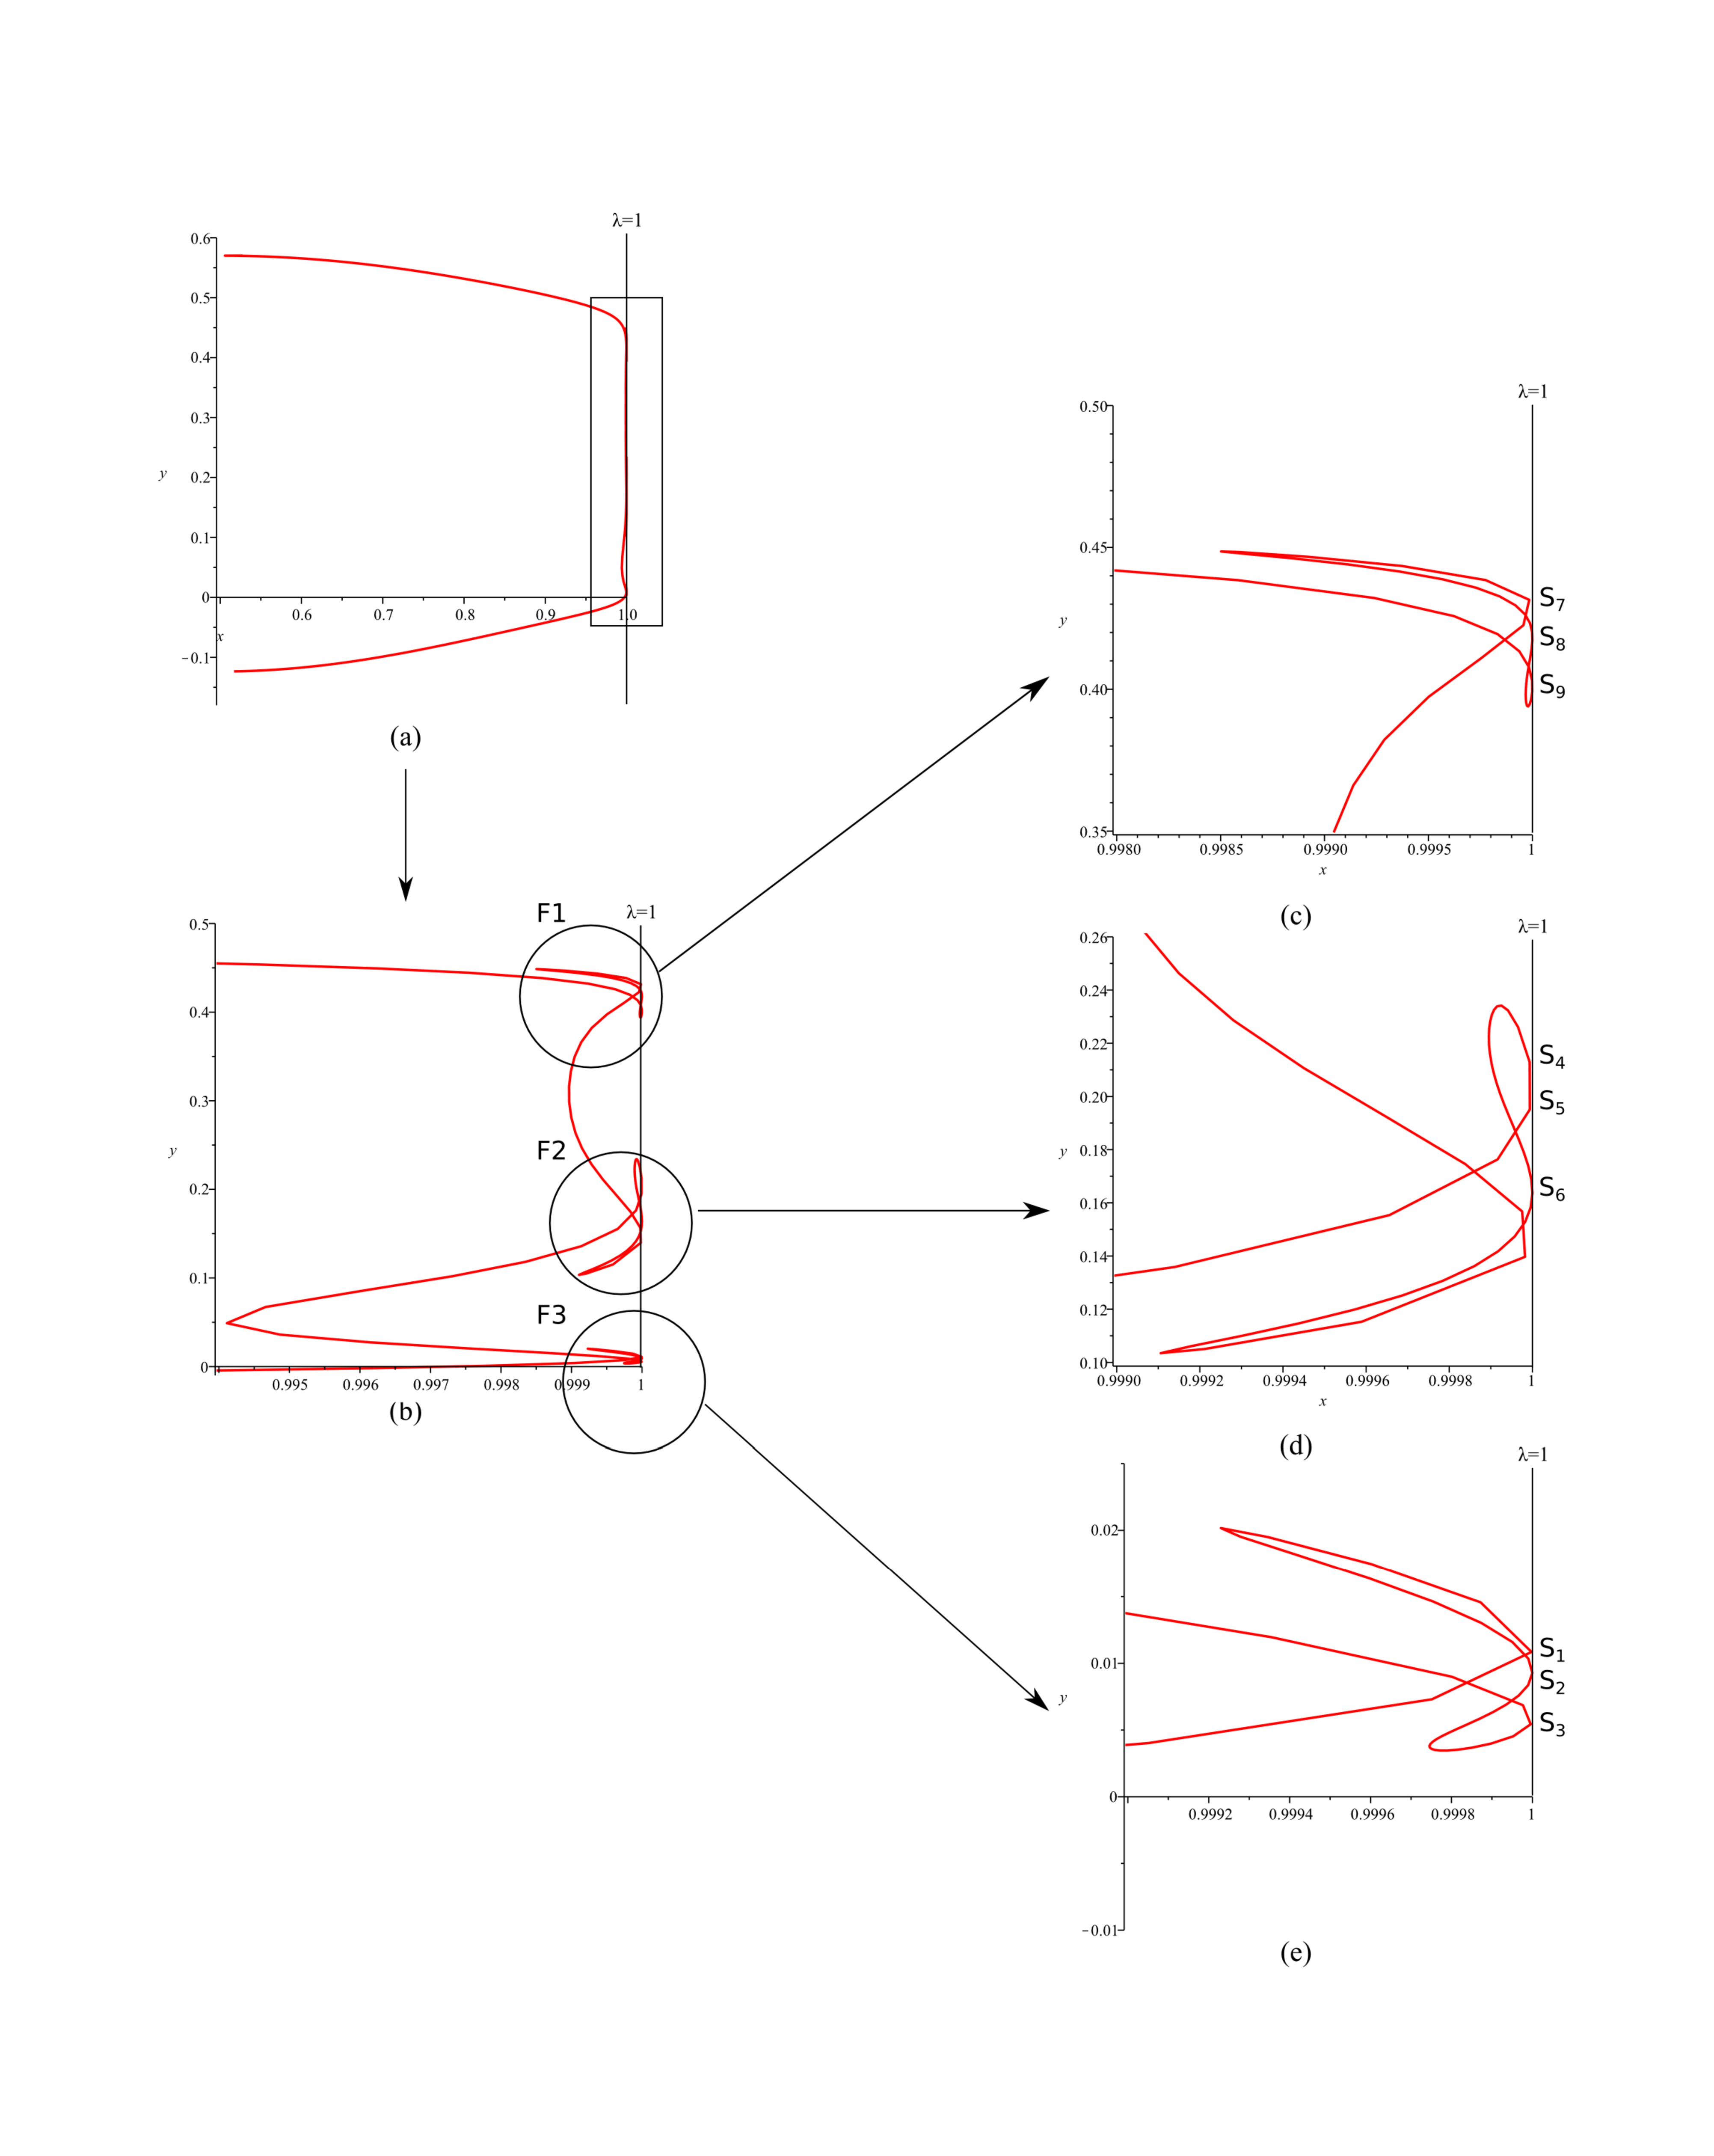
\includegraphics[scale=0.25]{figs/2diodos/group.eps} 
}
\caption{Homotopy path for tunnel diode circuit.}
\label{2tunelg}
\end{figure}

The numerical continuation scheme is broken down for this example, this way the numerical details for the tracing are shown. The trace starts at the symmetry axis at the point:

\begin{displaymath}
\begin{array}{r}
\left[\begin{array}{r} I_E \\ v_2  \\ v_3  \\ \lambda  \\
\end{array}\right]
\begin{array}{r}
 \\ = \\ \\ \end{array}
\left[\begin{array}{r}
-7.955452 \\
-0.123579  \\
-0.149062 \\
0.50000 \\
\end{array}\right]
\end{array}
\end{displaymath}

Root detection is achieved monitoring the sing change for $\Delta \lambda$ on each predictor step of the numerical continuation. Points obtained from this monitoring are $x_A$, $x_B$ and $x_C$, which are employed to interpolate the solution value $x_P$ at $\lambda=1$. Once interpolated the root, point $x_P$ is used as initial point for the NR method, this way the operating point  $x_s$ is located with higher precision. Also, the previous process is repeated for each solution $x_s$. In table \ref{detectaraices} the complete interpolation and tuning process is shown for each operating point $x_s$ of the circuit with two tunnel diodes.

\begin{table*}[tbp]
{
\center{
\begin{tabular}{||c|c|c||}
\hline\hline
Interpolation points  & Solution point $x_s$  \\ 
 $x=[I_d,u_2,u_3]$           &  Interpolated ($x_P$) en $\lambda=1$ & en $\lambda=1$    \\ \hline\hline
\begin{tabular}{c} 
 $x_A=[0.034309, 0.007303 , 0.003806]$ \\ 
$x_B=[0.047491, 0.010853 , 0.010434]$ \\ 
$x_C=[0.059196, 0.014573 , 0.018749]$  \end{tabular} & [0.048874, 0.011261 , 0.011261] & $S_1=[0.053618, 0.012688 , 0.014306]$  \\ \hline 
   \begin{tabular}{c} 
 $x_A=[0.045773, 0.010357 , 0.135764]$ \\ 
$x_B=[0.041903, 0.009283 , 0.148002]$ \\ 
$x_C=[0.038452, 0.008360 , 0.160252]$  \end{tabular} & [0.042176, 0.009354 , 0.147132] & $S_2=[0.041994, 0.009307 , 0.147695]$ \\ \hline 
   \begin{tabular}{c} 
 $x_A=[0.022494, 0.004530 , 0.413618]$ \\ 
$x_B=[0.026494, 0.005433 , 0.424871]$ \\ 
$x_C=[0.032519, 0.006861 , 0.435502]$  \end{tabular} & [0.028280, 0.005847 , 0.428548] & $S_3=[0.029835, 0.006213 , 0.431889]$ \\ \hline 
   \begin{tabular}{c} 
 $x_A=[0.028194, 0.176319 , 0.435376]$ \\ 
$x_B=[0.021433, 0.195091 , 0.424153]$ \\ 
$x_C=[0.016390, 0.212876 , 0.410115]$  \end{tabular} & [0.018920, 0.203419 , 0.418183] & $S_4=[0.018149, 0.206252 , 0.415641]$ \\ \hline 
   \begin{tabular}{c} 
 $x_A=[0.031351, 0.168846 , 0.172506]$ \\
$x_B=[0.033565, 0.163650 , 0.163498]$ \\ 
$x_C=[0.032428, 0.158301 , 0.154487]$  \end{tabular} & [0.033614, 0.163863 , 0.163863] & $S_5=[0.033258, 0.165521 , 0.166704]$ \\ \hline 
   \begin{tabular}{c} 
 $x_A=[0.023509, 0.115270 , 0.024727]$ \\ 
$x_B=[0.038392, 0.139699 , 0.011749]$ \\ 
$x_C=[0.046565, 0.156731 , 0.006817]$  \end{tabular} & [0.042176, 0.147132 , 0.009354] & $S_6=[0.043461, 0.149907 , 0.008475]$ \\ \hline 
\begin{tabular}{c} 
 $x_A=[0.035023, 0.422566 , 0.003153]$ \\ 
$x_B=[0.031774, 0.431522 , 0.007603]$ \\ 
$x_C=[0.041815, 0.438497 , 0.013568]$  \end{tabular} & [0.028280, 0.428548 , 0.005847] & $S_7=[0.032042, 0.425881 , 0.004447]$ \\ \hline 
   \begin{tabular}{c} 
 $x_A=[0.020448, 0.420201 , 0.194475]$ \\ 
$x_B=[0.018228, 0.417211 , 0.207798]$ \\ 
$x_C=[0.016335, 0.414336 , 0.221108]$  \end{tabular} & [0.018920, 0.418183 , 0.203419] & $S_8=[0.019650, 0.419203 , 0.198810]$\\ \hline 
   \begin{tabular}{c} 
 $x_A=[0.008437, 0.396283 , 0.385859]$ \\ 
$x_B=[0.009317, 0.399111 , 0.396140]$ \\ 
$x_C=[0.010717, 0.403016 , 0.405827]$  \end{tabular} & [0.009914, 0.400856 , 0.400856] & $S_9=[0.010303, 0.401943 , 0.403876]$ \\ \hline
\end{tabular}
}
\caption{Root detection by rebound on the solution line.}
\label{detectaraices}
}
\end{table*} 

Once the path tracing has crossed all nine solutions, it goes towards the symmetry axis, at this moment the crossing through the symmetry axis is monitored, as a consequence the simulation is stopped. The crossing is detected on the following points $x_E$ and $x_F$:

{
\begin{displaymath}
x_E=
\begin{array}{r}
\left[\begin{array}{r} I_d \\ u_2  \\ u_3  \\ \lambda  \\
\end{array}\right]
\begin{array}{r}
 \\ = \\ \\ \end{array}
\left[\begin{array}{r}
8.021018 \\
0.570133  \\
0.587474 \\
0.503422 \\
\end{array}\right]
\end{array} \\\\\\\\
, \qquad x_F=
\begin{array}{r}
\left[\begin{array}{r} I_d \\ u_2  \\ u_3  \\ \lambda  \\
\end{array}\right]
\begin{array}{r}
 \\ = \\ \\ \end{array}
\left[\begin{array}{r}
8.033125 \\
0.570171 \\
0.587512 \\
0.491161\\
\end{array}\right]
\end{array}
\end{displaymath}
}

\subsection{Circuit with four bipolar transistors and one diode}

This circuit was reported in \cite{homo_tadeusiewicz} and \cite{homo_yamamurawise}; it was solved using piecewise methods. Later, in \cite{homo_yamamura}, the circuit was solved using modified fixed point Homotopy. This circuit has three operating points. The Ebers-Moll model \cite{homo_ebersmoll} is employed for all transistors. The model equation is given as:

\begin{displaymath}
\left[ \begin{array}{c}
i_{D_E} \\
i_{D_C}
\end{array}\right] =
\left[ \begin{array}{cc} 1  & \alpha_R \\
\alpha_F & 1 \\
\end{array}\right] \left[ \begin{array}{c}
10^{-9}(e^{(40v_{be})} - 1) \\
10^{-9}(e^{(40v_{bc})} - 1)
\end{array}\right]
\end{displaymath}

The circuital rendering of the model is shown in figure \ref{FEbersMoll}.

The diode model is:

\begin{displaymath}
i_d=10^{-9}(e^{40u} - 1)
\end{displaymath}

In figure \ref{yamamuracircuito} the circuit is shown and equation \ref{eqsd} shows the non-linear equation system from the circuit (using the MNA circuit analysis method).

{\tiny
\begin{equation}
\begin{array}{r}
{\frac {37}{20000}}\,{\it v_1}-{\frac {1}{4000}}\,{\it v_2}-{\frac {1}{
 4000}}\,{\it v_6}-{\frac {1}{1000}}\,{\it v_9}-{\frac {1}{4000}}\,{\it 
v_{12}}-{\frac {1}{10000}}\,{\it v_{13}}+{\it IE}=0 \\
-{\frac {1}{4000}}\,{\it v_1}+{\frac {3}{8000}}\,{\it v_2}-{\frac {1}{
8000}}\,{\it v_5}+ 0.00000000990\,{{\rm e}^{40\,{\it v_4}-40\,{\it v_3}}}
+ 0.00000000010- 0.000000010\,{{\rm e}^{40\,{\it v_4}-40\,{\it v_2}}}=0  \\
{\frac {1}{100}}\,{\it v_3}- 0.000000010\,{{\rm e}^{40\,{\it v_4}-40\,{
\it v_3}}}+ 0.00000000990+ 0.00000000010\,{{\rm e}^{40\,{\it v_4}-40\,{
\it v_2}}}=0 \\
{\frac {1}{8000}}\,{\it v_4}-{\frac {1}{8000}}\,{\it v_6}+ 0.00000000010
\,{{\rm e}^{40\,{\it v_4}-40\,{\it v_3}}}- 0.00000001000+ 0.00000000990
\,{{\rm e}^{40\,{\it v_4}-40\,{\it v_2}}}=0 \\
-{\frac {1}{8000}}\,{\it v_2}+{\frac {1}{8000}}\,{\it v_5}+
 0.00000000010\,{{\rm e}^{40\,{\it v_5}-40\,{\it v_7}}}- 0.00000001000+
 0.00000000990\,{{\rm e}^{40\,{\it v_5}-40\,{\it v_6}}}=0 \\
-{\frac {1}{4000}}\,{\it v_1}-{\frac {1}{8000}}\,{\it v_4}+{\frac {3}{
8000}}\,{\it v_6}+ 0.00000000990\,{{\rm e}^{40\,{\it v_5}-40\,{\it v_7}}}
+ 0.00000001010- 0.000000010\,{{\rm e}^{40\,{\it v_5}-40\,{\it v_6}}}-
 0.000000010\,{{\rm e}^{40\,{\it v_8}-40\,{\it v_6}}}=0 \\
{\frac {1}{100}}\,{\it v_7}- 0.000000010\,{{\rm e}^{40\,{\it v_5}-40\,{
\it v_7}}}+ 0.00000000990+ 0.00000000010\,{{\rm e}^{40\,{\it v_5}-40\,{
\it v_6}}}=0 \\
{\frac {1}{30000}}\,{\it v_8}-{\frac {1}{30000}}\,{\it v_9}+ 0.000000010
\,{{\rm e}^{40\,{\it v_8}-40\,{\it v_6}}}- 0.000000010=0 \\
-{\frac {1}{1000}}\,{\it v_1}-{\frac {1}{30000}}\,{\it v_8}+{\frac {31}{
30000}}\,{\it v_9}+ 0.00000000990\,{{\rm e}^{40\,{\it v_{11}}-40\,{\it v_{10}
}}}+ 0.00000000010- 0.000000010\,{{\rm e}^{40\,{\it v_{11}}-40\,{\it v_9}}
}=0 \\
{\frac {1}{100}}\,{\it v_{10}}- 0.000000010\,{{\rm e}^{40\,{\it v_{11}}-40\,
{\it v_{10}}}}+ 0.00000000990+ 0.00000000010\,{{\rm e}^{40\,{\it v_{11}}-40
\,{\it v_9}}}=0 \\
{\frac {1}{10000}}\,{\it v_{11}}-{\frac {1}{10000}}\,{\it v_{12}}+
 0.00000000010\,{{\rm e}^{40\,{\it v_{11}}-40\,{\it v_{10}}}}- 0.00000001000
+ 0.00000000990\,{{\rm e}^{40\,{\it v_{11}}-40\,{\it v_9}}}=0 \\
-{\frac {1}{4000}}\,{\it v_1}-{\frac {1}{10000}}\,{\it v_{11}}+{\frac {7}{
20000}}\,{\it v_{12}}+ 0.00000000990\,{{\rm e}^{40\,{\it v_{13}}}}+
 0.00000000010- 0.000000010\,{{\rm e}^{40\,{\it v_{13}}-40\,{\it v_{12}}}}=0 \\
-{\frac {1}{10000}}\,{\it v_1}+{\frac {11}{10000}}\,{\it v_{13}}+
 0.00000000010\,{{\rm e}^{40\,{\it v_{13}}}}- 0.00000001000+
 0.00000000990\,{{\rm e}^{40\,{\it v_{13}}-40\,{\it v_{12}}}}=0 \\
 v_1-12=0\\
\end{array}
\label{eqsd}
\end{equation}}

\begin{figure*}[tbp]
\centerline{
\epsfxsize=100mm
\epsffile{chap4/figs/diotran.eps}
}
\caption{Circuit with four bipolar transistors and one diode.}
\label{yamamuracircuito}
\end{figure*}

\begin{figure}[hbtp]
\psfrag{f}{$\alpha_F$}
\psfrag{r}{$\alpha_R$}
\centerline{
\epsfxsize=26mm
\epsffile{chap4/figs/ebersmoll.eps}}
\caption{Ebers-Moll bipolar transistor model.}
\label{FEbersMoll}
\end{figure}

The values for the circuit components are found in table \ref{yamamuracircuitovalores}. First, the equilibrium formula is found using the modified nodal analysis, the analysis shows that the system has 14 variables.

\begin{table}[hbtp]
\center{
{\scriptsize
\begin{tabular}{||c|c||}
\hline\hline
Component  & Value  \\ \hline\hline
$R_1$ & $4K\Omega$   \\ \hline
$R_2$ & $0.1K\Omega$   \\ \hline
$R_3$ & $8K\Omega$   \\ \hline
$R_4$ & $8K\Omega$   \\ \hline
$R_5$ & $4K\Omega$   \\ \hline
$R_6$ & $0.1K\Omega$   \\ \hline
$R_7$ & $30K\Omega$   \\ \hline
$R_8$ & $1K\Omega$   \\ \hline
$R_9$ & $0.1K\Omega$   \\ \hline
$R_{10}$ & $10K\Omega$   \\ \hline
$R_{11}$ & $4K\Omega$   \\ \hline
$R_{12}$ & $10K\Omega$   \\ \hline
$R_{13}$ & $1K\Omega$   \\ \hline
$V_{cc}$ & $12V$   \\ \hline  \hline
\end{tabular}
}
}
\caption{Values for the resistors employed.}
\label{yamamuracircuitovalores}
\end{table}

Then, the circuit is solved using double bounded Homotopy (using $a=0$, $b=1$, $C=1$ and $D=1940$), the result showed the three solutions for the system. These solutions are shown in table \ref{yamamuracircuitosoluc1}, where $S_1$, and $S_3$ are stable and $S_2$ is unstable. Besides, table \ref{yamamuracircuitosoluc1} includes the initial point $x_i$ and final point $x_f$ of the path.
Finally, The Homotopy path corresponding to nodal voltage $v_2$ is shown in figure \ref{yamaie}.

\begin{table*}[tbp]
{\tiny
\center{
\hspace{-4mm}
\begin{tabular}{||c|c|c|c|c|c|c|c|c|c|c|c|c|c|c|c||}
\hline\hline
Relevant Points & $v_1$ & $v_2$ & $v_3$ & $v_4$ & $v_5$ & $v_6$ & $v_7$ & $v_8$ & $v_9$ & $v_{10}$& $v_{11}$ & $v_{12}$ & $v_{13}$ & $i_E$  & $\lambda$\\ \hline
$x_i$ &  11.99 & -15.41 &  -1.42 & -15.04 & -127.15 & 40.22 & -1.40 & -420.75 & -1.71 & -1.41 & -1.35 & -0.34 & 0.32 & -0.03 & 0.5 \\ \hline
$S_1+$ & 12 & 0.405 & 0.366 &0.685 &0.349 &6.796 &0.070 &7.038 &11.839 &0.4e-5 &0.039 &0.039 &0.321 &-0.0085 & 1 \\ \hline 
$S_2-$ & 12 & 0.883 & 0.278 &0.590 &0.631 &0.812 &0.315 &1.074 &11.647 &0.4e-5 &0.039 &0.039 &0.321 &-0.0100 & 1\\ \hline
$S_3+$ &  12 & 5.995 & 0.085 &0.368 &0.712 &0.436 &0.390 &0.699 &11.635 &0.4e-5 &0.039 &0.039 &0.321 &-0.0089 &1 \\ \hline 
$x_f$ &  11.99 & 0.84 &  0.83 & 1.20 & -110.90&  45.64 & -1.40 &  -420.73 &  -1.71 &  1.38 &  -1.35 &  -0.034 &  0.32 & -0.03 & 0.5 \\ \hline \hline
\end{tabular}
}
}
\caption{Homotopy path: relevant points)}
\label{yamamuracircuitosoluc1}
\end{table*}


\begin{figure}[hbtp]
\centerline{
\epsfxsize=70mm
\epsffile{chuayamamura/yamav2a.eps}
\epsfxsize=70mm
\epsffile{chuayamamura/yamav2b.eps}
}
\caption{Homotopy path of Yamamura's circuit for $v_2$}
\label{yamaie}
\end{figure}

\subsection{Chua's circuit}

Chua's circuit (see figure \ref{chua}), which has nine solutions, has become the benchmark for Homotopies applied to circuits. The values for the components are shown in table \ref{chuatablet}. This circuit has four bipolar transistors modeled by the Ebers-Moll model for bipolar transistor working in the direct active region (see figure \ref{eber}).

\begin{table}[hbtp]
\center{
{\scriptsize
\begin{tabular}{||c|c|c|c||}
\hline\hline
Component  & Value  & Component & Value\\ \hline\hline
$R_1$ & $1k\Omega$ & $R_9$ & $10.1k\Omega$    \\ \hline
$R_2$ & $4k\Omega$ & $R_{10}$ & $10.1k\Omega$  \\ \hline
$R_3$ & $4k\Omega$  &  $R_{11}$ & $4k\Omega$  \\ \hline
$R_4$ & $5k\Omega$  &  $R_{12}$ & $4k\Omega$  \\ \hline
$R_5$ &  $30k\Omega$ & $R_{13}$ & $30k\Omega$    \\ \hline
$R_6$  & $0.5k\Omega$ & $R_{14}$ & $30k\Omega$  \\ \hline
$R_7$ & $0.5k\Omega$  &  $V_1$ & $10V$  \\ \hline
$R_8$ & $30k\Omega$  &  $V_2$ & $2V$  \\ \hline
$V_{CC}$ & $12V$  &  $\alpha$& $0.98$     \\ \hline\hline
\end{tabular}
}
}
\caption{Chua's circuit component values.}
\label{chuatablet}
\end{table}

\begin{figure}[hbtp]
\centerline{
\epsfxsize=70mm
\epsffile{chap4/figs/chua.eps}}
\caption{Chua's circuit with nine solutions.}
\label{chua}
\end{figure}

\begin{figure}[hbtp]
\psfrag{F}{{\tiny $I_D=10^{-9}(e^{40v_D}-1)$}}
\psfrag{b}{{\tiny $\alpha=0.98$}}
\centerline{
\epsfxsize=35mm
\epsffile{chap4/figs/eber.eps}}
\caption{Ebers-Moll half-side model.}
\label{eber}
\end{figure}

The equation system is:

\begin{displaymath}
{\small
\begin{array}{l}
f_1=4.3663v_2+0.6103168 \times 10^{-5} e^{(40v_1)}-12+0.2863168\times 10^{-5}e^{(40v_2)}=0 \\ \\
f_2=5.4v_1+v_3+0.3580\times 10^{-5}e^{(40v_1)}-22+7\times 10^{-7}e^{(40v_3)}+  5\times 10^{-7}e^{(40v_4)}+0.6620\times 10^{-5}e^{(40v_2)}=0 \\ \\
f_3=4.3663v_4+0.6103168\times 10^{-5}e^{(40v_3)}-12+0.2863168\times 10^{-5}e^{(40v_4)}=0 \\
\end{array}
}
\end{displaymath}

The equilibrium equation is the same employed in \cite{homo_chua}. The variables to solve are branch voltages: $v_1$, $v_2$, $v_3$, and $v_4$. Figure \ref{chuaf} presents the Homotopy path against branch voltage $v_1$. This Homotopy method found six out of nine solutions (using $a=0$, $b=1$, $C=1$ and $D=0.0001$); the three remaining roots were isolated in a separate path.

\begin{figure}[hbtp]
\centerline{
\epsfxsize=40mm
\epsffile{chuayamamura/chuaa.eps}
\epsfxsize=40mm
\epsffile{chuayamamura/chuab.eps}
\epsfxsize=40mm
\epsffile{chuayamamura/chuac.eps}
}
\caption{Chua's circuit graphical solution.}
\label{chuaf}
\end{figure}

The initial point is $x_i=[0.400, 0.389, 0.399, 0.393]$ and final point is $x_f=[-10.353,0.425,-38.771,0.425]$ of the homotopy path, where the homotopy parameter is $\lambda=0.5$.
Finally, the solutions found are (where $\lambda=1$):

\begin{displaymath}
\begin{array}{r}
Solutions=
\left[\begin{array}{r}
v_1 \\ v_2  \\ v_3  \\ v_4  \\
\end{array}\right]
\begin{array}{r}
 \\ = \\ \\ \end{array}
\underbrace{\left[\begin{array}{r}
-1.0510 \\ 0.3775 \\  0.3845\\  -3.9542 \\
\end{array}\right]}_{\mbox{Solution \ding{172}}},
\underbrace{\left[\begin{array}{r}
-0.7119\\0.3775\\ 0.3350\\ 0.3653 \\ 
\end{array}\right]}_{\mbox{Solution \ding{173}}},
\underbrace{\left[\begin{array}{r}
-0.5136\\0.3775\\-0.9682\\0.3775\\
\end{array}\right]}_{\mbox{Solution \ding{174}}}, \\\\
\underbrace{\left[\begin{array}{r}
0.3242\\0.3703\\ -1.0395\\0.3775 \\
\end{array}\right]}_{\mbox{Solution \ding{175}}},
\underbrace{\left[\begin{array}{r}
0.3300 \\ 0.3680 \\ 0.3367 \\ 0.3642 \\
\end{array}\right]}_{\mbox{Solution \ding{176}}},
\underbrace{\left[\begin{array}{r}
0.3369\\ 0.3641\\0.3836\\-3.7069 \\
\end{array}\right]}_{\mbox{Solution \ding{177}}},
\end{array}
\end{displaymath}

\section{Conclusions}

In general terms, the stop criterion in Homotpy methods consist in the use of a maximum number (arbitrary number) of integration steps, such that when integration steps reach the solution line boundary the algorithm stops. Nevertheless, this kind of method could have roots left to find. The result of this investigation has been the definition of a new kind of Homotopy, which has an automatic stop criterion, as a consequence of the qualitative properties (symmetry and bounding) of the Homotopy paths. It was explained and developed a group of properties for each one of its parts. Double bounded Homotopy shows new and interesting properties. Because  allows the Homotopy path be placed between two limits named bounding lines. Also, the curved radius for the solutions shows a proportional relationship with the separation of solution lines. Besides, the curved radius for the turning points coincides spatially with the critical points for the equilibrium equation and directly proportional to $f(x)$ evaluated at return. Another fundamental property for this new Homotopy is having a symmetry axis placed between boundary lines, allowing to implement the stop criterion. Finally, double bounded Homotopy was applied to the simulation in DC for some circuits showing its potential for the analysis of non-linear circuits.

\bibliographystyle{amsplain}
\bibliography{nuevah}

\end{document}